% !TeX program = pdflatex
% !TeX spellcheck = en_US
% !TeX encoding = UTF-8
% !BIB program = biber

% v1.10 - 2017-05-30
% - Erik: Refactor the file structure of the front pages
% - Erik: Fix double bibliography entry
% v1.9 - 2017-02-03
% - Dirk: fixed warning: Underfull \hbox (badness 10000) in paragraph main.tex
% - Dirk: fixed warning: "Data encoding is UTF8" -> style.tex 0.1.8
% v1.8 - 2017-02-02
% - Dirk: replaced titlesec package by KOMA-script commands.-> style.tex v0.1.7
% v1.7 - 2014-11-18
% - bib fixes: now using biber instead of bibtex (thanks felix)
% - compile now with pdflatex -> biber -> pdflatex
% v1.6 - 2013-05-13
% - bibliography headers fixed - thanx lorenz lehmann
% - high quality titlepage - thanx thomas graf
% - removed separation of online and offline references -> style 1.4a
% v1.5 - 2013-01-16

\documentclass[twoside,11pt,titlepage,a4paper,english,bibliography=totocnumbered,listof=numbered]{scrbook}
%
% Template Style
% =========================================================================
% = SNET THESIS TEMPLATE STYLE
% =========================================================================

% http://www.snet.tu-berlin.de
% ------------------------
% Adapted version from http://hci.rwth-aachen.de/karrer_thesistemplate (Thorsten Karrer)
% Further adaptions for http://www.elearn.rwth-aachen.de (Sascha Hoellger)
% Further adaptions for SNET @ TU Berlin by Sebastian Göndör (sebastian.goendoer@tu-berlin.de)


% =========================================================================
% = CHANGELOG
% =========================================================================
% [0.1.9]
% - Fixed styling for chapters and toc using Komascript
% - Remove double bibliography TOC entry
%
% [0.1.8]
% - fixed "warning UFT8 is used". biblatex requires ascii encoding; by Dirk
%
% [0.1.7]
% replaced "Titelsec" commands (and whole package) by appropriate KOMA-Script commands; by Dirk
%
% [0.1.6]
% replaced deprecated \rm commands with \rmfamily commands; by Dirk
%
% [0.1.4b]
% backend=biber added in line 139
%
% [0.1.4a]
% title page: image logo sizes and margins adjusted to printable area
% removed separation of online and offline references
%
% [0.1.3]
% wider text body
% added "school" to the titlepage
% paragraph indents
% correctly placed footnote graphics
%
% [0.1.2]
% new titlepage
% some minor fixes
%
% [0.1.1]
% changed titlepage logo
% added listoffigures and listoftables
% excluded abstract from toc
% no (roman) numbering for frontmatter
%
% [0.1]
% adapted version 0.991b from sascha hoellger @ rwth aachen


% =========================================================================
% = MISC
% =========================================================================

\usepackage{a4wide}					%
\usepackage{verbatim}				%
\usepackage[toc,page]{appendix}			%
\usepackage[withpage]{acronym}			%
\usepackage{amsthm}				% Definitions


% =========================================================================
% = COLORS
% =========================================================================

\usepackage{xcolor}					% Colors
\definecolor{LightBlue}{rgb}{0.55,0.55,1}
\definecolor{DarkBlue}{rgb}{0.2,0.2,0.5}
\definecolor{DarkRed}{rgb}{0.71,0.12,0.07}

% =========================================================================
% = PAGE LAYOUT
% =========================================================================

\usepackage{geometry}
\geometry{inner=3cm, outer=2cm, bottom=4cm}

\newcommand{\setwidesite}				% changes the geometry to have less margin
{
	\fancyhfoffset[LE,RO]{0cm}
	\fancyheadoffset[LO,RE]{0cm}
	\fancyfootoffset[RE]{2cm}
	\newgeometry{inner=2cm, outer=2cm, bottom=4cm}
}

\usepackage{style/noindent}				%do not indent at new paragraphs but add a vertical offset

\setlength{\parindent}{4mm}
\setlength{\parskip}{1.5mm }


% =========================================================================
% = TYPESETTING
% =========================================================================

\usepackage[hyphens]{url}				% url
\usepackage{hyphenat}				% hyphenation. use \hyphenation{}

\righthyphenmin=5
\lefthyphenmin=5


% =========================================================================
% = TABLE OF CONTENTS
% =========================================================================

\setcounter{secnumdepth}{4}
\setcounter{tocdepth}{3}

\addtokomafont{disposition}{\rmfamily}


% =========================================================================
% = FONTS
% =========================================================================

\usepackage{mathpazo}
\usepackage[scaled=.95]{helvet}
\usepackage{courier}


% =========================================================================
% = SYMBOLS
% =========================================================================

%\usepackage{gensymb}
\usepackage{textcomp} 				% for \textmu (non-italic $\mu$)
\makeatletter						% this makes "@" a regular letter


% =========================================================================
% = TABLES
% =========================================================================

\usepackage{tabularx}
\usepackage{booktabs}
\usepackage{multirow}
\usepackage{longtable}				% tables spanning over more than one page

%%\setlength{\fboxsep}{0mm}			% spacing between \fbox border and content

\usepackage{amsmath}				% math fonts
\usepackage{amssymb}				% math symbols
\usepackage{setspace}				% line spacing


% =========================================================================
% = BIBILOGRAPHY
% =========================================================================

\usepackage[style=numeric,natbib=true,backend=biber,sorting=none]{biblatex}

% apparently no effect?
%\renewcommand{\bibsetup}{
%	\markboth{
%		\MakeUppercase{Bibliography}
%	}{}
%}

\ifdefined\bibheadingonline
  \defbibheading{online}{\section*{\bibheadingonline}}
\else
  \defbibheading{online}{\section*{Online References}}
\fi
\ifdefined\bibheadingoffline
  \defbibheading{offline}{\section*{\bibheadingoffline}}
\else
  \defbibheading{offline}{\section*{Printed References}}
\fi

\defbibfilter{online}{%
  \( \type{online} \)}

\defbibfilter{offline}{%
  \( \not \type{online} \)}

\bibliography{bibliography}


% =========================================================================
% = LANGUAGE & ENCODING
% =========================================================================

\usepackage[english]{babel}				% \usepackage[ngerman]{babel}

\selectlanguage{english}				% \selectlanguage{ngerman}

\usepackage[T1]{fontenc}
\usepackage[utf8]{inputenc}				% can use native umlauts

% \usepackage[babel,german=quotes]{csquotes}	% provides \enquote{Blupp} => "`Blupp"'
\usepackage[babel,english=american]{csquotes}	% provides \enquote{Blupp} => "`Blupp"'

\SetCiteCommand{\parencite}			% Changed for biblatex

\usepackage{units}					% unified way of setting values with units

\usepackage{appendix}


% =========================================================================
% = CODE LISTINGS
% =========================================================================

\usepackage{listings}

% Listings Styles from Max

\definecolor{violet}{cmyk}{0.45,0.97,0.27,0.21}
\definecolor{lstblue}{cmyk}{1,0.80,0,0}
\definecolor{lstgreen}{cmyk}{0.71,0.21,0.65,0.22}
\definecolor{bluegrey}{cmyk}{0.56,0.24,0.11,0.05}
\definecolor{javadoc}{cmyk}{0.88,0.59,0,0}
\definecolor{lstgrey}{cmyk}{0.55,0.44,0.42,0.32}

\lstdefinelanguage{SQL}{
     keywords={},
     keywordstyle=\color{bluegrey}\bfseries,
     morekeywords=[2]{CREATE,TABLE,IF,NOT,EXISTS,NULL,SET,DEFAULT,PRIMARY,KEY,COLLATE,CHARACTER,AUTO_INCREMENT,ENGINE,CHARSET},
     keywordstyle={[2]\color{violet}\bfseries},
     otherkeywords={int,varchar,double,text,tinyint},
     sensitive=false,
     morecomment=[l][\color{lstgreen}]{//},
     morecomment=[s][\color{lstgreen}]{/*}{*/},
     morecomment=[s][\color{javadoc}]{/**}{*/},
     morestring=[b]',
     morestring=[b]"
  }
\lstdefinelanguage{PHP}{
     keywords={},
     keywordstyle=\color{bluegrey}\bfseries,
     morekeywords=[2]{static,function,if,return,pow,sin,cos,asin,min,sqrt,int},
     keywordstyle={[2]\color{violet}\bfseries},
     otherkeywords={@param, @returns, @author, @type, @link, @see},
     sensitive=false,
     morecomment=[l][\color{lstgreen}]{//},
     morecomment=[s][\color{lstgreen}]{/*}{*/},
     morecomment=[s][\color{javadoc}]{/**}{*/},
     morestring=[b]',
     morestring=[b]"
  }
\lstdefinelanguage{JavaScript}{
     keywords={},
     keywordstyle=\color{bluegrey}\bfseries,
     morekeywords=[2]{attributes, class, classend, do, empty, endif, endwhile, fail, function, functionend, if, implements, in, inherit, inout, not, of, operations, out, return, set, then, types, while, use},
     keywordstyle={[2]\color{violet}\bfseries},
     otherkeywords={@param, @returns, @author, @type, @link, @see},
     sensitive=false,
     morecomment=[l][\color{lstgreen}]{//},
     morecomment=[s][\color{lstgreen}]{/*}{*/},
     morecomment=[s][\color{javadoc}]{/**}{*/},
     morestring=[b]',
     morestring=[b]"
  }
\lstdefinelanguage{Java}{
     keywords={},
     keywordstyle=\color{bluegrey}\bfseries,
     morekeywords=[2]{abstract,boolean,break,byte,case,catch,char,class,
      const,continue,default,do,double,else,extends,false,final,
      finally,float,for,goto,if,implements,import,instanceof,int,
      interface,label,long,native,new,null,package,private,protected,
      public,return,short,static,super,switch,synchronized,this,throw,
      throws,transient,true,try,void,volatile,while},
     keywordstyle={[2]\color{violet}\bfseries},
     morekeywords=[3]{@SuppressWarnings, @Capability, @Override},
     keywordstyle={[3]\color{lstgrey}},
     otherkeywords={@param, @return, @returns, @author, @link, @see},
     sensitive,
     morecomment=[l]//,
     morecomment=[s]{/*}{*/},
     morecomment=[s][\color{javadoc}]{/**}{*/},
     morestring=[b]",
     morestring=[b]',
  }[keywords,comments,strings]

% some listings styles from Gregor Aisch
% http://vis4.net/blog/2009/09/noch-mehr-sprach-definitionen-fuer-latex-listings/

\lstdefinelanguage{HTML5} {morekeywords={a, abbr, address, area, article, aside, audio, b, base, bb, bdo, blockquote,  body, br, button, canvas, caption, cite, code, col, colgroup, command, datagrid, datalist, dd, del, details, dialog, dfn, div, dl, dt, em, embed, eventsource, fieldset, figure, footer,  form,  h1, h2,  h3,  h4, h5,  h6,  head,  header,  hr, html,  i, iframe,  img,  input,  ins, kbd,  label,  legend,  li,  link,  mark,  map,  menu,  meta,  meter,  nav,  noscript,  object,  ol,  optgroup,  option,  output,  p,  param,  pre,  progress,  q,  ruby,  rp,  rt,  samp,  script,  section,  select,  small,  source,  span,  strong,  style,  sub,  sup,  table,  tbody,  td,  textarea,  tfoot,  th,  thead,  time,  title,  tr,  ul,  var,  video},
sensitive=false, morecomment=[s]{<!--}{-->}, morestring=[b]", morestring=[d]'}

\lstdefinelanguage{CSS} {morekeywords={azimuth,  background-attachment,  background-color,  background-image,  background-position,  background-repeat,  background,  border-collapse,  border-color,  border-spacing,  border-style,  border-top, border-right, border-bottom, border-left,  border-top-color, border-right-color, border-bottom-color, border-left-color,  border-top-style, border-right-style, border-bottom-style, border-left-style,  border-top-width, border-right-width, border-bottom-width, border-left-width,  border-width,  border,  bottom,  caption-side,  clear,  clip,  color,  content,  counter-increment,  counter-reset,  cue-after,  cue-before,  cue,  cursor,  direction,  display,  elevation,  empty-cells,  float,  font-family,  font-size,  font-style,  font-variant,  font-weight,  font,  height,  left,  letter-spacing,  line-height,  list-style-image,  list-style-position,  list-style-type,  list-style,  margin-right, margin-left,  margin-top, margin-bottom,  margin,  max-height,  max-width,  min-height,  min-width,  orphans,  outline-color,  outline-style,  outline-width,  outline,  overflow,  padding-top, padding-right, padding-bottom, padding-left,  padding,  page-break-after,  page-break-before,  page-break-inside,  pause-after,  pause-before,  pause,  pitch-range,  pitch,  play-during,  position,  quotes,  richness,  right,  speak-header,  speak-numeral,  speak-punctuation,  speak,  speech-rate,  stress,  table-layout,  text-align,  text-decoration,  text-indent,  text-transform,  top,  unicode-bidi,  vertical-align,  visibility,  voice-family,  volume,  white-space,  widows,  width,  word-spacing,  z-index},
sensitive=false, morecomment=[s]{/*}{*/}, morestring=[b]", morestring=[d]'}

\lstdefinelanguage{JavaFX} {morekeywords={abstract, after, and, as, assert, at, attribute, before, bind, bound, break, catch, class, continue, def, delete, else, exclusive, extends, false, finally, first, for, from, function, if, import, indexof, in, init, insert, instanceof, into, inverse, last, lazy, mixin, mod, new, not, null, on, or, override, package, postinit, private, protected, public-init, public, public-read, replace, return, reverse, sizeof, static, step, super, then, this, throw, trigger, true, try, tween, typeof, var, where, while, with },
sensitive=false, morecomment=[l]{//}, morecomment=[s]{/*}{*/}, morestring=[b]", morestring=[d]'}

\lstdefinelanguage{MXML} {morekeywords={mx:Accordion, mx:Box, mx:Canvas, mx:ControlBar, mx:DividedBox, mx:Form, mx:FormHeading, mx:FormItem, mx:Grid, mx:GridItem, mx:GridRow, mx:HBox, mx:HDividedBox, mx:LinkBar, mx:Panel, mx:TabBar, mx:TabNavigator, mx:Tile, mx:TitleWindow, mx:VBox, mx:VDividedBox, mx:ViewStack, mx:Button, mx:CheckBox, mx:ComboBase, mx:ComboBox, mx:DataGrid, mx:DateChooser, mx:DateField, mx:HRule, mx:Image, mx:Label, mx:Link, mx:List, mx:Loader, mx:MediaController, mx:MediaDisplay, mx:MediaPlayback, mx:MenuBar, mx:NumericStepper, mx:ProgressBar, mx:RadioButton, mx:RadioButtonGroup, mx:Spacer, mx:Text, mx:TextArea, mx:TextInput, mx:Tree, mx:VRule, mx:VScrollBar, mx:Application, mx:Repeater, mx:UIComponent, mx:UIObject, mx:View, mx:FlexExtension, mx:UIComponentExtension, mx:UIObjectExtension, mx:Fade, mx:Move, mx:Parallel, mx:Pause, mx:Resize, mx:Sequence, mx:WipeDown, mx:WipeLeft, mx:WipeRight, mx:WipeUp, mx:Zoom, mx:EventDispatcher, mx:LowLevelEvents, mx:UIEventDispatcher, mx:CurrencyFormatter, mx:DateFormatter, mx:NumberFormatter, mx:PhoneFormatter, mx:ZipCodeFormatter, mx:CursorManager, mx:DepthManager, mx:DragManager, mx:FocusManager, mx:HistoryManager, mx:LayoutManager, mx:OverlappedWindows, mx:PopUpManager, mx:SystemManager, mx:TooltipManager, mx:CreditCardValidator, mx:DateValidator, mx:EmailValidator, mx:NumberValidator, mx:PhoneNumberValidator, mx:SocialSecurityValidator, mx:StringValidator, mx:ZipCodeValidator, mx:DownloadProgressBar, mx:ArrayUtil, mx:ClassUtil, mx:Delegate, mx:ObjectCopy, mx:URLUtil, mx:XMLUtil, mx:CSSSetStyle, mx:CSSStyleDeclaration, mx:CSSTextStyles, mx:StyleManager, mx:HTTPService, mx:RemoteObject, mx:Service},
sensitive=false, morecomment=[s]{<!--}{-->}, morestring=[b]", morestring=[d]'}

\lstdefinelanguage{LZX} {morekeywords={a, alert, animator, animatorgroup , attribute, audio , axis, axisstyle , b, barchart, basebutton , basebuttonrepeater , basecombobox , basecomponent , basedatacombobox , basedatepicker , basedatepickerday , basedatepickerweek , basefloatinglist , basefocusview , baseform , baseformitem , basegrid , basegridcolumn , baselist , baselistitem , basescrollarrow , basescrollbar , basescrollthumb , basescrolltrack , baseslider , basestyle , basetab , basetabelement , basetabpane , basetabs , basetabsbar , basetabscontent , basetabslider , basetrackgroup , basetree , basevaluecomponent , basewindow , br , button , canvas , chart , chartbgstyle , chartstyle , checkbox , class , columnchart , combobox , command , connection , connectiondatasource , constantboundslayout , constantlayout , datacolumn , datacombobox , datalabel , datamarker , datapath , datapointer , dataselectionmanager , dataseries , dataset , datasource , datastyle , datastylelist , datatip , datepicker , debug , dragstate , drawview , edittext , event , face , floatinglist , font , font , form , frame , grid , gridcolumn , gridtext , handler , hbox , horizontalaxis , hscrollbar , i , image , img , import , include , inputtext , javarpc , label , labelstyle , layout , legend , library , linechart , linestyle , list , listitem , LzTextFormat , menu , menubar , menuitem , menuseparator , method , modaldialog , multistatebutton , node , p , param , piechart , piechartplotarea , plainfloatinglist , plotstyle , pointstyle , pre , radiobutton , radiogroup , rectangularchart , regionstyle , remotecall , resizelayout , resizestate , resource , reverselayout , richinputtext , rpc , script , scrollbar , security , selectionmanager , sessionrpc , simpleboundslayout , simpleinputtext , simplelayout , slider , soap , splash , stableborderlayout , state , statictext , style , submit , swatchview , SyncTester , tab , tabelement , tabpane , tabs , tabsbar , tabscontent , tabslider , Test , TestCase , TestResult , TestSuite , text , textlistitem , tickstyle , tree , u , valueline , valuelinestyle , valuepoints , valuepointstyle , valueregion , valueregionstyle , vbox , verticalaxis , view , view , vscrollbar , webapprpc , window , windowpanel , wrappinglayout , XMLHttpRequest , xmlrpc , zoomarea},
sensitive=false, morecomment=[s]{<!--}{-->}, morestring=[b]", morestring=[d]'}

\lstset{
  numbers=left,
  numberstyle=\tiny,
  numbersep=5pt,
  breaklines=true,
  stepnumber=1,
  tabsize=2,
  basicstyle=\ttfamily\small,
  frame=none,
  numberfirstline=true,
  firstnumber=1,
  keywordstyle=\color{violet}\bfseries,
  ndkeywordstyle=\color{bluegrey}\bfseries,
  identifierstyle=\color{black},
  commentstyle=\color{lstgreen}\ttfamily,
  stringstyle=\color{lstblue}\ttfamily,
  showstringspaces=false
}


% ========================================================================
% = CHANGE LIST DEFINITIONS
% ========================================================================

% change color of item list
\renewcommand{\labelitemi}{\color{DarkRed}$\bullet$}
\renewcommand{\labelitemii}{\color{DarkRed}$\circ$}
\renewcommand{\labelitemiii}{\color{DarkRed}$\ast$}
\renewcommand{\labelitemiv}{\color{DarkRed}$\diamond$}

% change color of enum list
\renewcommand{\labelenumi}{\color{DarkRed}\arabic{enumi}.}
\renewcommand{\labelenumii}{\color{DarkRed}\alph{enumii})}
\renewcommand{\labelenumiii}{\color{DarkRed}\roman{enumiii}.}
\renewcommand{\labelenumiv}{\color{DarkRed}\Alph{enumiv}.}

% change color of description list
\usepackage{enumitem}
\setdescription{font=\color{DarkRed}\rmfamily\itshape}
% \renewenvironment{description}{\list{font=\color{DarkRed}\itshape}}{\endlist}


% ========================================================================
% = FOOTNOTES
% ========================================================================

% change color of footnotes
\renewcommand{\thefootnote}{\color{DarkRed}\arabic{footnote}}

% use nice footnote indentation
\deffootnote[1em]{1em}{1em}{\textsuperscript{\thefootnotemark}\,}


% =========================================================================
% = GRAPHICS AND IMAGES
% =========================================================================

\usepackage{graphicx}
\graphicspath{{images/}}				% path to your image folder

\usepackage{eso-pic}					% needed for the full-face titlepage
\usepackage{chngpage}				% we need this to determine if a figure is on an odd or even page
\usepackage{tikz}					% tikz pictures

% captions of tables and images
\usepackage[hang,small,sf]{caption}
\renewcommand{\captionfont}{\rmfamily\small}
\renewcommand{\captionlabelfont}{\bfseries}

\usepackage{float}
\usepackage{placeins}
% \floatstyle{ruled}
%\floatplacement

\renewcommand{\floatpagefraction}{0.85}		% if a figure takes more than 85% of a page it will be typeset on a separate page
\usepackage[it,bf,tight,hang,raggedright]{subfigure}

%\numberwithin{figure}{section}
%\numberwithin{table}{section}


% =========================================================================
% = HEADER
% =========================================================================

\newcommand{\STYLEfootnotetext}
{
  \begin{minipage}
  {.2\textwidth}
    
\includegraphics[width=0.9\textwidth]{images/snet/snet_footer.png}
  \end{minipage}
}

% Change page headers and footers:
\usepackage{calc}
\usepackage{fancyhdr}
\pagestyle{fancy}
\fancyhfoffset[RO,LE]{0.1cm} %{\marginparsep+\marginparwidth}
\fancyhfoffset[RE,LO]{0.1cm}
%\fancyheadoffset[RE,LO]{\hoffset + \oddsidemargin}
\renewcommand{\headrule}{{\color{DarkRed}%
  \hrule width\headwidth height\headrulewidth \vskip-\headrulewidth}}
\fancyhf{}
\fancyhead[RE]{\slshape \nouppercase{\leftmark}}    % Even page header: "page   chapter"
\fancyhead[LO]{\slshape \nouppercase{\rightmark}}   % Odd  page header: "section   page"
\fancyhead[RO,LE]{\bfseries \thepage}

%- \fancyfoot[LE]{\STYLEleftpicture}
%- \fancyfoot[RO]{\STYLErightpicture}
\fancyfoot[LE]{\STYLEfootnotetext}

\renewcommand{\headrulewidth}{1pt}    % Underline headers
\renewcommand{\footrulewidth}{0pt}

% =========================================================================
% = SECTIONS THEMING
% =========================================================================

\newcommand{\allsectionformat}{\color{DarkRed}\rmfamily\normalfont}

% Font style and colors
\addtokomafont{part}{\Huge\allsectionformat}
\addtokomafont{chapter}{\Huge\allsectionformat}
\addtokomafont{section}{\allsectionformat}
\addtokomafont{subsection}{\allsectionformat}
\addtokomafont{subsubsection}{\allsectionformat}
\addtokomafont{paragraph}{\allsectionformat}
\addtokomafont{subparagraph}{\allsectionformat}

% Spacing before and after the section titles
\RedeclareSectionCommand[
  beforeskip=-.75\baselineskip,
  afterskip=.5\baselineskip]{section}

\RedeclareSectionCommand[
  beforeskip=-5\baselineskip,
  afterskip=.5\baselineskip]{chapter}


% =========================================================================
% = TYPESETTING - TWEAKES
% =========================================================================

\addtokomafont{section}{\LARGE}
\addtokomafont{subsection}{\large}

% instead of sloppy
%\tolerance 1414
%\hbadness 1414
%- \tolerance 2414
%- \hbadness 2414
%- \emergencystretch 1.5em
%- \hfuzz 0.3pt
%- \widowpenalty=10000     % Hurenkinde r
%- \clubpenalty=10000      % Schusterjungen
%- \brokenpenalty=10000
%- \interlinepenalty=9000 % seitenumbruch im absatz
%- \vfuzz \hfuzz
%- \raggedbottom


% =========================================================================
% =  USER DEFINED COMMANDS
% =========================================================================

\newcommand{\chapterquote}[2]{
    \begin{quotation}
    \begin{flushright}
    \noindent\emph{``{#1}''\\[1.5ex]---{#2}}
    \end{flushright}
    \end{quotation}
}


% ==========================================================================
% = ALGORITHMS
% ==========================================================================
\usepackage[linesnumbered, ruled, vlined]{algorithm2e}
\usepackage{algpseudocode}

% ==========================================================================
% = ENUMARATE WITH ALPHABETS
% ==========================================================================
\usepackage{enumitem}

% ==========================================================================
% = REMOVES TAB IN PARAGRAPHS
% ==========================================================================
\usepackage[parfill]{parskip}
\addbibresource{bibliography.bib}

% custom hyphenation					% add words to this list to prevent hyphenation
\hyphenation{
ASCII
TCP
}

%make readable references
\usepackage[pdftex,pdfpagelabels=true,hyperfootnotes=false,driverfallback=dvipdfm]{hyperref}
\usepackage{float}
\hypersetup{%
	pdftitle={Community Detection in Large-scale Networks},
	pdfauthor={Dalwar Hossain},
	pdfkeywords={Community Detection, Large-scale Networks, Graph Theory},
	pdfsubject={Digital Communities},
	colorlinks=true,
	citecolor=red,
	linkcolor=blue,
	urlcolor=blue
}

\renewcommand{\thefootnote}{\textcolor{red}{\arabic{footnote}}}
% Adding a finite stretch on the page suppresses "Underfull \vbox (badness 10000)" warnings.
\makeatletter
\def\@textbottom{\vskip \z@ \@plus 1pt}
\let\@texttop\relax
\makeatother

\begin{document}

%--------------------------------------------------------------
% FRONT PAGE AND DOCUMENT METADATA
%--------------------------------------------------------------
\frontmatter

\begin{titlepage}
	\AddToShipoutPicture*{
		\put(0,0){
			
\includegraphics[width=\paperwidth,height=\paperheight,keepaspectratio=false]{images/snet/titlepage.pdf}
		}
	}
	\strut
	\hfill
	\begin{center}
	\vspace{1cm}
		\Huge
		\begin{spacing}{.9}
			\textcolor{DarkRed}{\textbf{Community Detection and Observation in Large-scale Transaction-based Networks}}\\
		\end{spacing}
		\vspace{0.8cm}
		\large
		by\\
		\vspace{0.8cm}
		\textbf{Dalwar Hossain}\\
		\vspace{0.2cm}
		Matriculation Number: \textbf{387610}\\
		\vspace{2cm}
	 	A thesis submitted to\\
		\vspace{0.5cm}
		Technische Universität Berlin\\
		School IV - Electrical Engineering and Computer Science\\
		Department of Telecommunication Systems\\
		Service-centric Networking\\
		\vspace{0.8cm}
		\textbf{Master Thesis}\\
		\vspace{1.8cm}
		\today\\
		\vspace{1.8cm}
		\large
		Supervised by:\\
		Prof. Dr. Axel Küpper\\
		\vspace{1cm}
		Assistant supervisor:\\
		Dr. Peter Ruppel\\
		Bianca Lüders\\
		\end{center}
\end{titlepage}

% Clear two pages after the title
\shipout\null
\shipout\null

\chapter*{\LARGE Eidestattliche Erklärung / Statutory Declaration}
Hiermit versichere ich, dass ich diese Arbeit selbst\-ständig verfasst und keine anderen als die angegebenen Quellen und Hilfsmittel benutzt habe.
\vspace{2em}

\noindent I hereby declare that I have created this work completely on my own and used no other sources or tools than the ones listed.

\vspace{30 mm}
\begin{flushright}

\rule{80mm}{1pt}

Berlin, \today \hspace{18 mm} Dalwar Hossain
\end{flushright}

%\chapter*{Acknowledgments}
\label{cha:acknowledgments}

This section is not visible on the PDF.

\chapter*{Abstract}
\label{cha:abstract}

Understanding community structures in a graph gives insight of the fundamental properties of a network by observing the characteristics and relationship between the nodes. This thesis will explore the state of the art community detection algorithms for large-scale networks preferably in blockchain/distributed ledger domain. As the popularity for both community detection and blockchain grows, research interest in respective domain grows simultaneously. Detecting community in large-scale network is challenging because of time and space complexity of the underlying algorithm and to observe change in the network requires additional approaches. This thesis proposes a prototypical framework for detecting community structures in blockchain data and observing changes in communities afterwards. All the implementation steps of the framework are clearly defined. It evaluates the framework in respect to time and space complexity with different well known community detection algorithms. It also proposes additional steps to observe changes in community at any given timestamp. This framework can be easily modified to suit the need of observing changes in any blockchain network. Significant improvement of this prototypical framework can be done in processing timestamped data-sets by using high end systems, parallel or distributed computing.

			% EN Abstract
\chapter*{Zusammenfassung}
\label{cha:zusammenfassung}

Das Verstehen von Gemeinschaftsstrukturen in einem Diagramm gibt einen Einblick in die grundlegenden Eigenschaften eines Netzwerks, indem die Eigenschaften und die Beziehung zwischen den Knoten beobachtet werden. Diese Dissertation wird die state of the art Community erkennungs algorithmen für große Netzwerke untersuchen, vorzugsweise im Blockchain / Distributed-Ledger-Bereich. Mit der wachsenden Beliebtheit von Community Detection und Blockchain wächst das Interesse an der jeweiligen Domain gleichzeitig. Das Erkennen von Communities in großen Netzwerken ist aufgrund der Komplexität von Zeit und Raum des zugrunde liegenden Algorithmus eine Herausforderung, und um Änderungen im Netzwerk zu beobachten, sind zusätzliche Ansätze erforderlich. Diese Arbeit schlägt einen prototypischen Rahmen vor, um Community-Strukturen in Blockchain-Daten aufzuspüren und danach Veränderungen in Communities zu beobachten. Alle Umsetzungsschritte des Rahmens sind klar definiert. Es bewertet das Framework in Bezug auf Zeit- und Raumkomplexität mit verschiedenen bekannten Community-Erkennungsalgorithmen. Es werden außerdem zusätzliche Schritte zum Beobachten von Änderungen in der Community zu einem bestimmten Zeitstempel vorgeschlagen. Dieses Framework kann leicht modifiziert werden, um Änderungen in einem Blockchain-Netzwerk zu beobachten. Eine signifikante Verbesserung dieses prototypischen Frameworks kann bei der Verarbeitung von Zeitstempeldatensätzen unter Verwendung von High-End-Systemen, paralleler oder verteilter Datenverarbeitung erreicht werden.	% DE Abstract

\tableofcontents{}

%--------------------------------------------------------------
% MAIN CONTENT
%--------------------------------------------------------------
\mainmatter

%\part{}						% optional: use parts to structure your thesis
\chapter{Introduction}\label{cha:1_introduction}
Recent development in networking has changed the way we think about complex systems. Researchers have concentrated their attention on a few properties that seem to be common in many real-life networks: the small-world property, power-law degree distributions and network transitivity \cite{ref-1}. One of the very challenging aspects of graphs in representing a real system is community structure. Recently, there is a growth in networks out of financial/asset transfer domains. These networks usually represent the business relationship between companies/agents. As a result, the graphs contain multiple edges between two same nodes as well as time stamps for each edge \cite{ref-19}. Analyzing the structure of a network allows us to better understand its fundamental properties by observing the characteristics and relationships between the vertices and edges of the corresponding graph. There is a growing number of distributed ledger/Blockchain-based networks that encompass the whole world and whose transaction lists are publicly accessible. Detecting community structures in massive graphs is challenging because of time and space complexity of the involved algorithms. In addition, previously identified community might change over time and might have added new transactions. Additional observation technique like birth, growth, splitting and death of communities are required to track and observe these dynamic communities \cite{ref-39}.

\section{Objectives}\label{objectives}
Finding community structures in massive networks is a growing and developing subject. The goal of this thesis is to design and develop a concept of a prototypical framework and implementation for detecting community structures and afterward observing changes in communities. The main focus of the thesis is on two complexity factors, run-time and memory management. The whole process revolves around the question "How well an approach performs on large-scale graphs?". To achieve the primary goal the following objectives had been set -
\begin{itemize}
	\item Provide an overview of state of the art community detection and observation in graphs.
	\item Conduct analysis of data sources, data types, and data concepts, preferably in the domain of Distributed Ledgers/Blockchain.
	\item Design a framework that can perform community detection and observation in large-scale transaction-based networks.
	\item Implement a prototype of the framework.
	\item Evaluate the performance (run-time and memory space requirements) of the framework.\footnote{Sample \textbf{Ethereum} data provided by SNET TU Berlin (\hyperlink{SNET-TUB}{http://www.snet.tu-berlin.de})}
\end{itemize}

This thesis focuses on the notion of community structures in blockchain network. It explores the idea that community structures exist in blockchain networks. Those community structures can be detected and monitored over time to observe the evolution of the network. For this purpose, a couple of community detection algorithm that can detect community structures in large-scale networks is tested against blockchain transaction data to determine the run-time and memory requirements. In the first chapter of this thesis, a brief introduction about communities, dynamic communities, community life-cycle, blockchain, why choosing blockchain for this thesis has been discussed. In the second chapter, an elaborate background study is discussed focusing on community detection techniques and their run-time and memory consumption. Also, the algorithms were explained in a fair manner later in chapter two. In chapter three of this thesis a prototypical framework for community structure detection and observation in large-scale network has been proposed and explained step by step. Implementation techniques and measures that have been used to test the run-time and memory consumption of the algorithms in the framework has been described in brief in chapter four. Chapter four also contains the evaluation, results and finding of the implementation. This thesis concludes with a few recommendations about future work that can be done in the field of blockchain with community detection and observation.

\section{What is a community in graph?}\label{community_in_graph}
Communities are groups of vertices which can easily be grouped together into set of nodes such that each set of node is densely connected internally and/or play similar roles within the graph \cite{ref-6}. Figure (\ref{fig:a_sample_community}) is an example of a sample graph that has three communities. Graphs representing real systems are not regular. They are objects where order coexists with disorder. The paradigm of disordered graph is the random graph \cite{ref-21}. Real networks are not random  graphs as the display big level of inhomogeneities, high level of order and organization. In real networks, the degree distribution is broad which most of the time follows power law \cite{ref-6}. As a result, many vertices with low degree coexists with some vertices with large degrees. Hence, the distribution of edges is not only globally but also locally inhomogeneous with high concentrations of edges within a special group of vertices and low concentration between these groups. This feature of real networks is called \textit{community structure} \cite{ref-1}.

\vfill
\pagebreak

\begin{figure}[H]
	\centering
	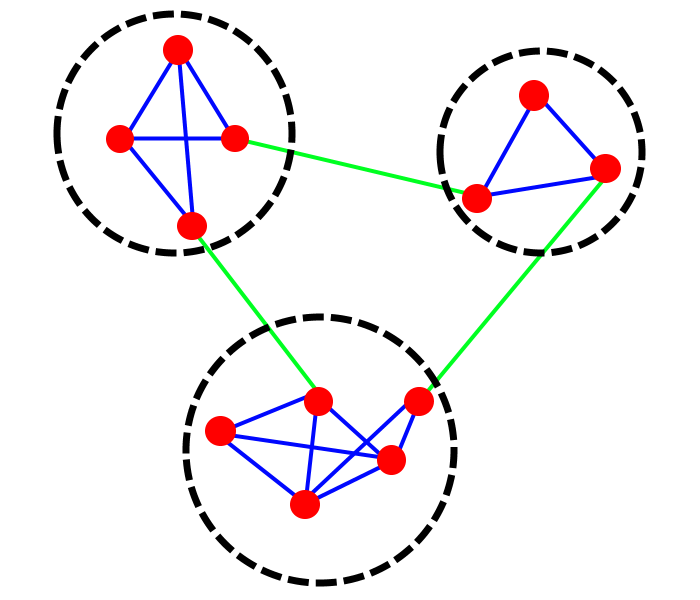
\includegraphics[width=0.5\textwidth]{community-sample}
	\caption{A graph with three communities, enclosed by dashed circles}
	\label{fig:a_sample_community}
\end{figure}

Society offers a wide range of possible groups of organizations: families, working and friendship circles, villages, towns, nations. Growth of Internet over the years also led us to the creation of virtual groups like online communities, forums and online gaming communities. Social communities have been studied for a long time \cite{ref-6}. Communities also occur in many networked systems from biology, computer science, engineering, economics, politics etc. In the graph of world wide web, they may correspond to groups of pages dealing with the same or related topics \cite{ref-36}.

Communities can have concrete applications. Clustering web clients who have similar interests and geographically near to each other may improve the performance of services provided on the world wide web, each cluster of clients can be served by a specific mirror server. Identifying clusters of customers with similar interests in the network of purchase relationship between customers and products of online retailers enables insight into customers' purchase behavior and also helps retailers to setup efficient recommendation systems \cite{ref-37}.

In every network, communities form because of some kind of interaction between nodes. In real life that could be interacting with each other. In animals that are being seen together or in a worldwide network, interaction between different system can produce community structures. In Figure (\ref{fig:communities_extra})(a), shows the famous Zachary's network of karate club members, a well-known graph regularly used in community detection benchmarking. It is consists of 34 nodes representing the 34 members of the club. It's visible from the figure that communities evolved around node 1, 33 and 34(the president of the club). The nodes in this network, inside a community is tightly connected as they represent social interaction between club members over 3 years of time period \cite{ref-58}.

Figure (\ref{fig:communities_extra})(b) shows the network of bottle-nose dolphins that were seen together more often. This also reflects the community structures in those dolphins. Figure (\ref{fig:communities_extra})(c) a relationship between AS (Autonomous Systems) form CAIDA project in 2007 is represented. It shows the interactions between different AS's. Nodes and their interactions with other AS is represented as edges and different colors represent different community structures.

\begin{figure}[H]
	\centering
	\begin{minipage}[b]{0.4\textwidth}
		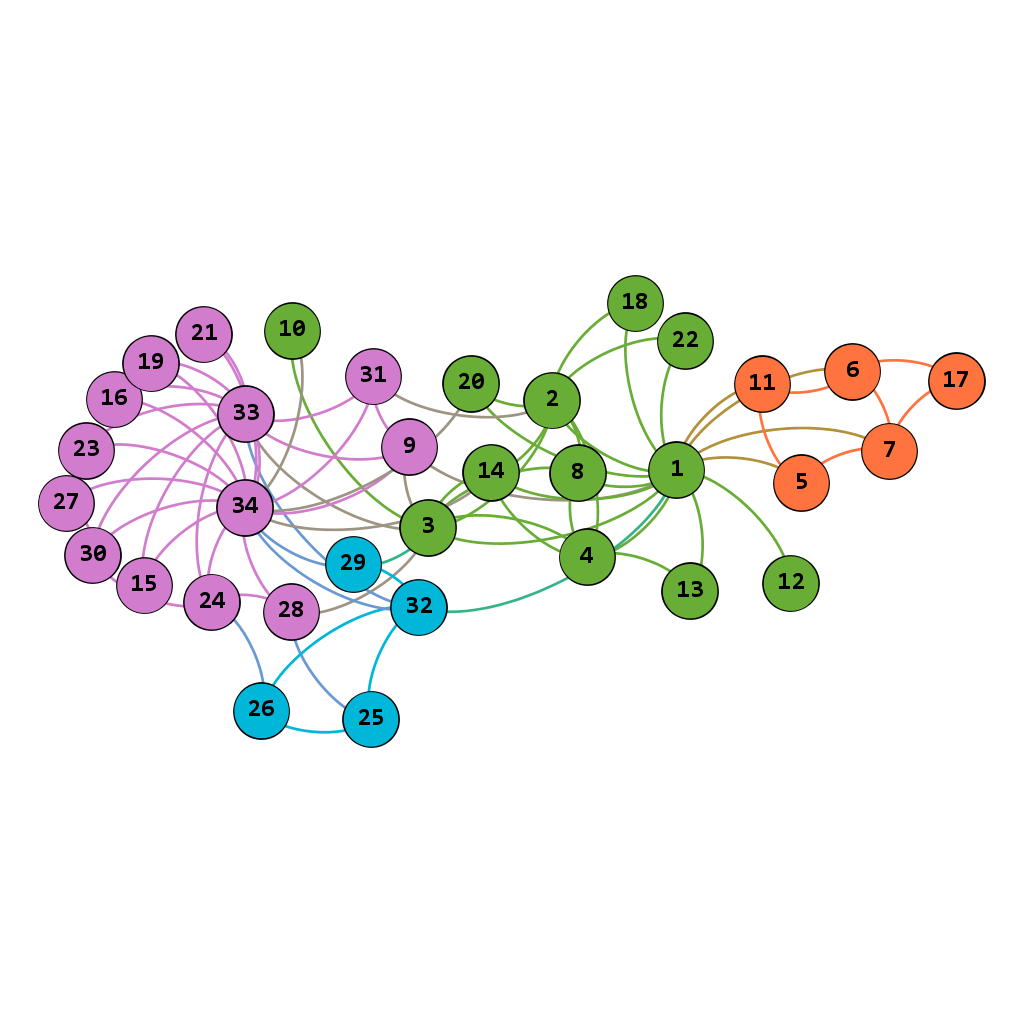
\includegraphics[width=\textwidth]{k_club_34}
		\caption*{(a)}
	\end{minipage}
	%\hfill
	\begin{minipage}[b]{0.4\textwidth}
		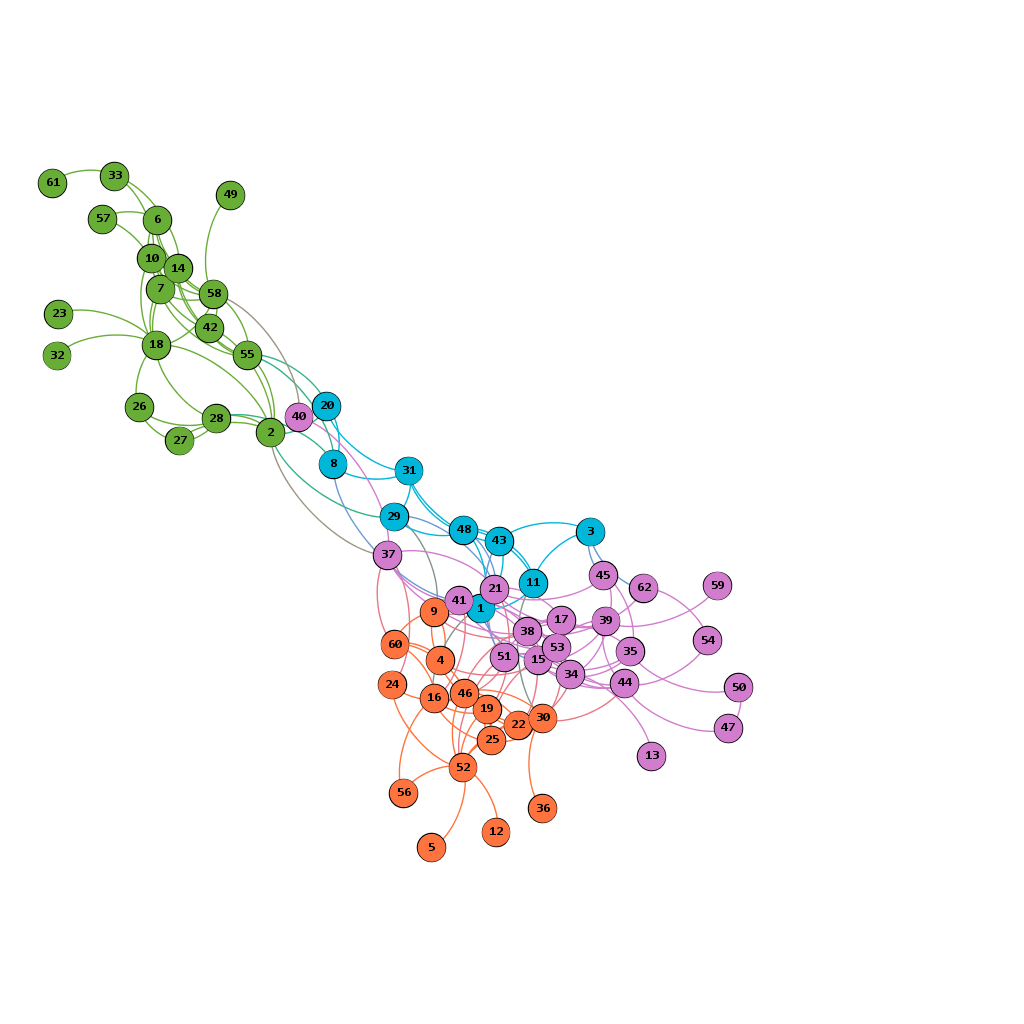
\includegraphics[width=\textwidth]{dolphins_62}
		\caption*{(b)}
	\end{minipage}
	%hfill
	\begin{minipage}[b]{0.8\textwidth}
		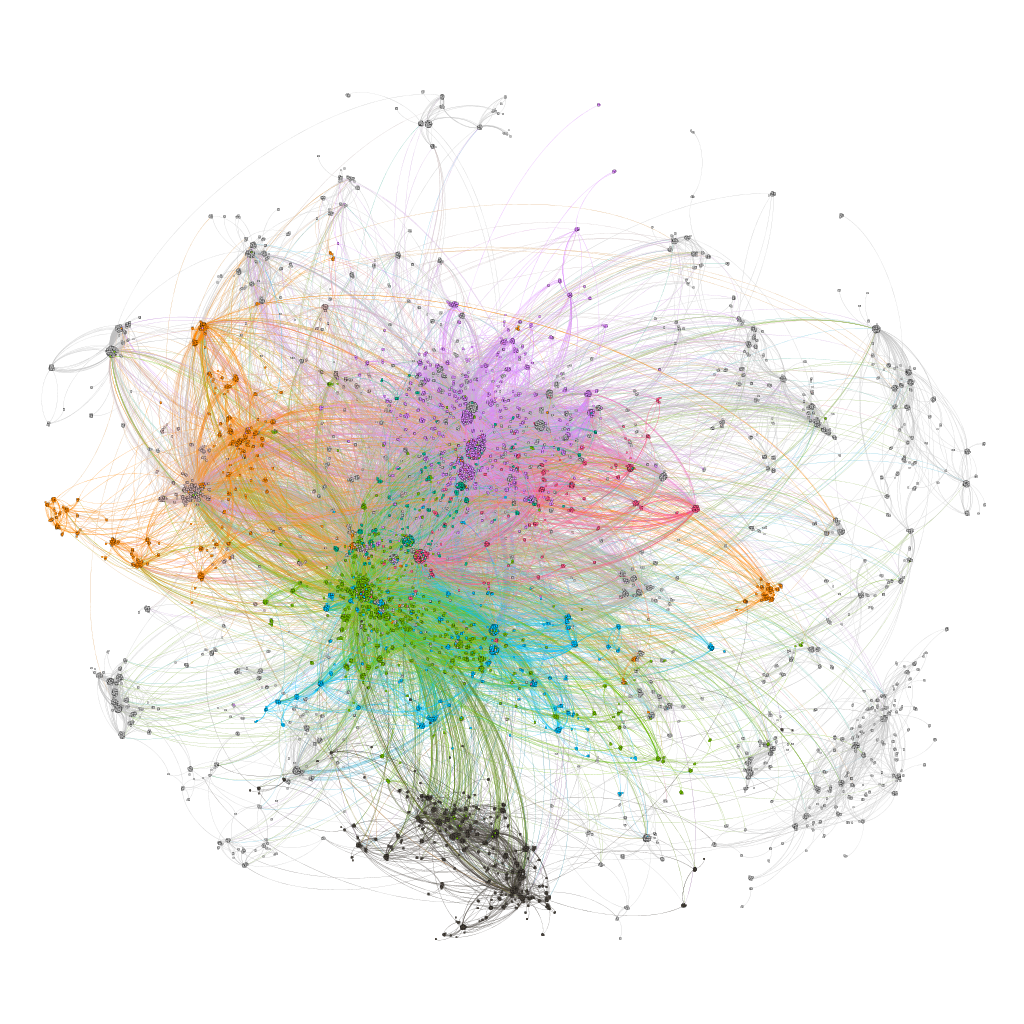
\includegraphics[width=\textwidth]{caida_26475}
		\caption*{(c)}
	\end{minipage}
	\caption{Community structures in different networks: (a) Famous Zachary's Karate club community structures. (b) Network of bottle nose dolphins (c) Community structures found in autonomous systems interaction with each other in CAIDA project in 2007}
	\label{fig:communities_extra}
\end{figure}

\section{Structure of Transaction-based Networks}
The use of network theory in transaction-based systems is relatively recent but it grew popular in the last few years. Since the data in transaction-based systems can be very different, the networks in transaction-based system are divided into similarity based networks and direct interaction networks. In similarity based networks, a link is drawn between two vertices if they share some features like strategy, behavior, income etc. This means that agents do not interact with each other but can be connected if they are similar. In direct interaction networks, a link between two nodes signals the presence of an interaction between the entities represented by the two nodes connected by the link. 

\subsection{Transaction Networks}
The most immediate application of networks to finance and economics is given whenever we have a transaction between two agents. The agents are the vertices and the transaction is the edge between them. In practice, the nodes represent banks and the weighted and directed edges represent a possible relation between banks. For transaction networks, two types of networks are considered to be most common. \textbf{First}, the inter-bank market and \textbf{Second}, payment system. Boss et al. in \cite{ref-20}, the inter-bank market is described as a network where the vertices given by the banks are nodes and the claim and liabilities between them are described as links. The inter-bank market is, therefore, a weighted and directed network.

\section{Distributed Ledger / Blockchain}
Blockchain is a distributed database solution that maintains a continuously growing list of data records that are confirmed by the nodes participating in it. Figure (\ref{fig:blockchain}) explains blockchain technology and it's different steps in the process of approving a transaction and adding a block of data to the root chain of blocks. The data is recorded in a public ledger, including information about every transaction ever completed. Blockchain is a decentralized solution which does not require any third party organization in the middle. The information about every transaction ever completed in Blockchain is shared and available to all nodes.
This attribute makes the system more transparent than centralized transactions involving a third party. In addition, the nodes in Blockchain are all pseudonymized, which makes it more secure for other nodes to confirm the transactions. Bitcoin was the first application that introduced Blockchain technology. Bitcoin created a decentralized environment for cryptocurrency, where the participants can buy and exchange goods with digital money \cite{ref-40}. A blockchain database is managed autonomously using a peer-to-peer network and a distributed time-stamping server. They are authenticated by mass collaboration powered by collective self-interests. The result is a robust work-flow where participants' uncertainty regarding data security is marginal.

\vfill
\pagebreak

\begin{figure}[H]
	\centering
	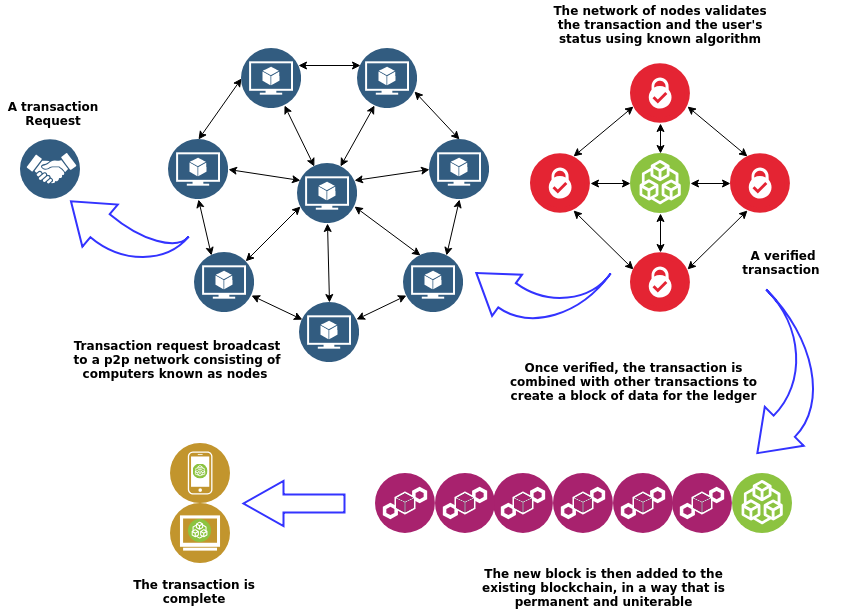
\includegraphics[width=\textwidth]{blockchain-explained}
	\caption{Blockchain explained}
	\label{fig:blockchain}
\end{figure}

\subsection{Why Blockchain?}
Blockchain is gaining popularity day by day for the past few years because of the security and anonymity it offers. Blockchain technology has allowed \textit{bitcoin} to flourish and become one of the most successful cryptocurrency over the years \cite{ref-41}. Blockchain transactions are worldwide and all the transaction data is public because it uses a distributed ledger system. It offers anonymity and irreversible, virtually unhackable security that protects transactions and assets. In Figure (\ref{fig:blockchain}), it shows that an approved block contains the hash of previous block and the previous block contains the hash it's previous block and so on. So to alter a block in the chain would be nearly impossible because to change one block, all the blocks needed to be changed and because it uses distributed ledger it's nearly impossible to get hold of all the ledger copies that are available over internet. There is also a business gain from ICO (Initial Coin Offering) from blockchain community for investing in different project. Its practically IPO (Initial Public Offering) on the basis of cryptocurrency. ICOs are changing how investors invest in and with cryptocurrency. So it's gaining popularity quick and people are getting more interested in buying cryptocurrency which leads to high value of cryptocurrency in the real world market. Blockchain technology is being used for asset transactions so it is a massive transaction-based network. For the scope of this thesis, blockchain is a suitable match as the transaction data is public, network is massive and transaction-based. Studying blockchain data and analyzing the network structure of blockchain will provide more deep insight about the properties of blockchain and network itself. It will also provide insight into business applications of blockchain. The security architecture can be better understood through community detection and observation. It will also help to learn how the transaction-based networking is changing over time allowing us to analyze the past transactions and predict future behavior of the network itself.

\section{Community Detection in Transaction-based Networks}
Recently the research on network-based graph theories has increased \cite{ref-1}. As a result, the complex and large-scale systems are being researched as well, based on different kinds of networks that exist in real-life. So to detect communities in a large-scale transaction-based systems, it is necessary to explore the idea of community, detection of community structures in large or massive graphs representing a system, characteristics of detecting communities in large-scale networks. It might also be necessary to explore additional techniques to actively monitor and keep track of previously detected community structures in a massive graph.

\subsection{Detection of Dynamic Community}\label{subsub:dynamic_community}
Community structures can change over time in transaction-based networks. It can have new nodes and new edges in between the existing nodes or can have new nodes connected to the old nodes through new edges. Those communities are actively changing its structure over time. It's a difficult and time consuming task to keep track of constantly changing communities. The analysis of dynamic communities is still in its infancy \cite{ref-6}. Studies in this direction have been mostly hindered by the fact that the problem of graph clustering is already controversial on single graph realizations, so it is understandable that most efforts still concentrate on the \textit{static} version of the problem. Another difficulty is represented by the dearth of time-stamped data on real graphs. Recently, several data-sets have become available, enabling to monitor the evolution in time of real systems \cite{ref-23}. So it has become possible to investigate how communities form, evolve and die. The main phenomena occurring in the lifetime of a community are in Figure (\ref{fig:community_evolution}): birth, growth, contraction, merger with other communities, split, death.

\vfill
\pagebreak

\begin{figure}[!ht]
	\centering
	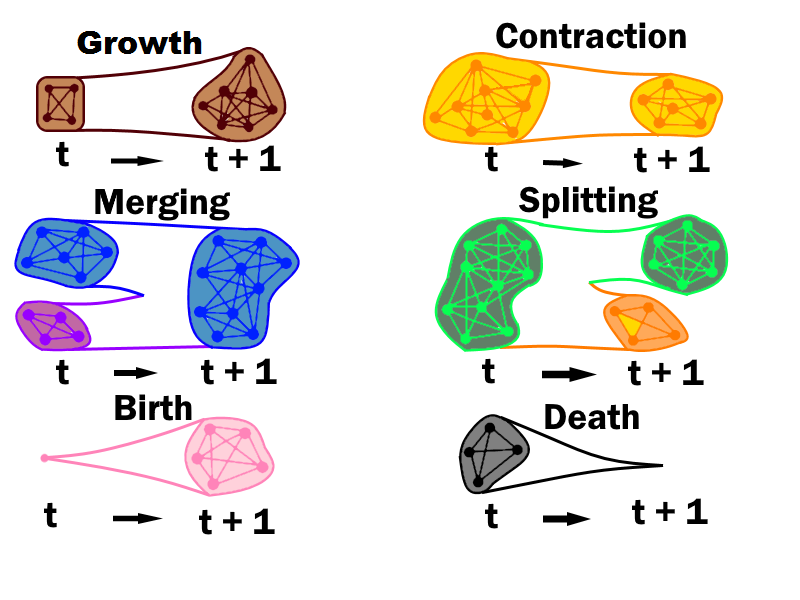
\includegraphics[width=0.7\textwidth]{community-evolution}
	\caption{Possible scenarios of community evolution \cite{ref-23}}
	\label{fig:community_evolution}
\end{figure}

One of the main objectives of this thesis is to explore and observe how community changes over the time and how to create a structured framework to track communities over time. Figure (\ref{fig:community_evolution}) is a good example of community changing over time. Community can get bigger or smaller, it can also split into different communities and can die.
\chapter{Related Work}\label{cha:2_relatedwork}
Section (\ref{community_in_graph}), describes in brief about community structures in graph and its similarities with real-life. This chapter of the thesis focuses on \textit{state of the art} community detection techniques and explains the algorithms in details. It also focuses on state of the art community detection algorithms and their complexity factors regarding run-time and space. Preceding literature of this chapter unfolds some of the widely used algorithms for community detection and also explores the complexity factors.

\section{Problems of community detection}
Mostly, two paradigms are used to discover the community structure of a network. One of them is based on the analysis of the global features of the network. We can consider network topology as an example. These approaches are characterized by high computational complexity and high-quality results. The other paradigm relies on the local information of the network. For an example of local information would be, information that is acquired by the nodes and their neighbors. The computational cost for these techniques is lower than those exploiting global features but the reliability decreases \cite{ref-28}.

Over the years many techniques have been proposed to detect community structures in large networks. There exist numerous comprehensive surveys of this problem such as \cite{ref-2}, \cite{ref-6}, \cite{ref-9}. The problem of finding communities in a network is intended as a data clustering problem. Two approaches have been widely investigated over the time for community detection in networks,
\begin{itemize}
	\item \textit{Spectral Clustering}
	\item \textit{Network Modularity Optimization} 
\end{itemize}
\textit{Spectral clustering} uses the optimization of the process of cutting the graph that represents the network and \textit{Modularity optimization} focuses on maximizing the modularity (quality function) of the network. For the first process, the problem of minimizing the number of cuts in a given graph has been proven to be NP-hard \cite{ref-29}. The main issue with spectral clustering based method is that one has to know in advance the number and the size of communities in a given graph representing a network. In large networks, this method is not feasible.

As for modularity optimization relies on a concept called network modularity. Network modularity is explained in details in this chapter earlier. Equation (\ref{sumoverclusters}) reveals a possible maximization strategy: in order to increase the value of first term, the highest possible number of edges should fall in each given community, whereas the minimization of the second term is obtained by dividing the network into several communities with small total degrees. The problem of maximizing the network modularity had been proven to be NP-Complete \cite{ref-30}. Several heuristic strategies have been proposed so far. (\ref{girvan-newman}) and (\ref{sub:fastalgorithm}) proposed by \textit{Girvan-Newman} are probably the most popular strategy to determine communities in a given graph representing a network. When considering a strategy to compute and detect communities, it's important to consider the resource needed and time for completing the computation. The computational cost for modularity maximization is high. It yields $\mathcal{O}(n^{3})$ where $n$ is the number of nodes. In this process, the largest part of the cost is given to calculate \textit{betweenness centrality}. Betweenness centrality is explained in brief in this chapter earlier in section (\ref{betweennesscentrality}).

Several variations of this strategy have been proposed and all of them were focused on faster calculation and detection on communities. The fast clustering algorithm by \textit{Clauset, Newman and Moore} \cite{ref-31}, that runs in $\mathcal{O}(n \log n)$ on sparse graphs; the external optimization method proposed by Duch and Arenas \cite{ref-32}, based on fast agglomerative approach, with $\mathcal{O}(n^2 \log n)$ time complexity; the Newman-Leicht \cite{ref-33} mixture model based on statistical inferences. Maximization techniques by Newman \cite{ref-34} based on eigenvectors and matrices.

\section{Literature Review}\label{sec:literature_review}
Over the past years, network research across the physical and social sciences grew very fast\cite{ref-25}. As a result, there are several techniques to determine community structure in a network. Finding communities within an arbitrary network can be a computationally difficult task. The number of communities, if any, within a network, is generally unknown and communities are often unequal in size or density. Despite these difficulties, however, several methods for community finding have been developed and employed with varying levels of success \cite{ref-2}. Following is a list of few well known community detection algorithms for large-scale networks and this chapter of the thesis is focused on technical aspects of these algorithms for community detection in large-scale networks.

\begin{enumerate}
	\item InfoMap
	\item Louvain Method
	\item Girvan-Newman algorithm
    \item Modularity maximization (Quality Function)
    \item Hierarchical clustering
	\item Graph partitioning
	\item Minimum cut method
	\item Statistical inference
	\item Clique-based methods
\end{enumerate}

These algorithms are chosen because of the nature of their performance against large-scale networks. According to the authors of these algorithms each one of them is fast and optimized for community detection. Authors of each algorithm have chosen different approach to detect communities in large-scale networks. Next section will attempt an ordered exposition of the fundamental concepts of some of these algorithms to explore the ideas and technical background behind these community detection algorithm in respect to large-scale transaction-based network. Although all the algorithm mentioned above are deemed fast enough at the time of their publications, some of them might not be suited for detecting community structures in large-scale transaction-based network. In chapter (\ref{cha:4_implementation_and_evaluation}), these algorithms will be evaluated with a prototypical framework for detecting communities in distributed ledger network.

\subsection{Infomap}\label{subsec:infomap}
Communities refer to groups of nodes that are densely connected internally. Community detection in networks is challenging, and many algorithms have been proposed in the last few years to tackle this difficult problem. The current implementation of Infomap is both fast and accurate \cite{ref-42}. It can classify millions of nodes in minutes and performs very well on synthetic data with planted communities. Furthermore, the map equation framework is also naturally flexible and can be straightforwardly generalized to analyze different kinds of network data \cite{ref-42}. Infomap uses, map equation \cite{ref-43} first introduced by Martin et. al in 2009. The map equation is a Flow-based method. Methods based on flows operate on the dynamics on the network rather than on its topological structure per se. The rationale is that the prime function of networks is to capture the flow between the components of the real systems they represent. Accordingly, communities consist of nodes among which flow persists for a long time once entered \cite{ref-42}. Map equation uses \textit{Huffman coding} \cite{ref-44} to send the location of the random walker \cite{ref-57} in the flow. Moreover, it is optimal for describing a list of locations of the random walker at arbitrary (and sufficiently distant) times. However, it can be used to list the locations visited by a random walker in a sequence of successive steps, after all this is the flow of the network \cite{ref-43}. 

\subsection{Louvain Method}\label{subsec:louvain_method}
\textit{Louvain Method} (henceforth, LM) was first introduced by Bodel et al. in 2008 in \cite{ref-27}. The authors in this publication proposed a simple method to extract the community structure of large networks. The proposed method is a heuristic method that is based on modularity optimization (\ref{sumoverclusters}). LM has outperformed all other known community detection methods in terms of computation time \cite{ref-28}. The subject of computation time of different community detection algorithms will be discussed in a comparative manner later in this chapter. Moreover, depending on modularity function, community detected by LM is very good. The authors introduced an algorithm that is capable of detecting high modularity partitions of large networks in a short time and it also unfolds a complete hierarchical community structure for the network. This unfolding process of unfolding structure gives access to different levels of resolutions of community detection. Authors have tested the algorithm with 118 million nodes network which took only 152 minutes\footnote{All methods described in \cite{ref-27} have been compiled and tested on the same machine: a biopteron
2.2k with 24GB of memory} \cite{ref-27}. In 2011, Meo et al. in \cite{ref-28} proposed a generalized LM for community detection in large network with a brief discussion of core LM \cite{ref-27} and with the help of the state of the art LM and $\mathcal{K}$-path edge centrality, message propagation and fast $\mathcal{K}$-path community detection. In this recent paper the authors have shown that their algorithm outperforms all the other community detection algorithms and also slightly improves the core LM \cite{ref-28}.

\subsection{Girvan-Newman Algorithm}\label{girvan-newman}
The most popular algorithm for community structure detection was proposed by Girvan and Newman \cite{ref-1}. This algorithm marked the new era in community detection. Here edges are selected according to the values of measures of \textit{edge centrality}, estimating the importance of the edge according to some property or process running on the graph. Girvan and Newman focused on the concept of \textit{betweenness} (\ref{betweennesscentrality}), which is a variable expressing the frequency of the participation of edges to a process. They considered three alternative definitions: \textit{geodesic edge betweenness}, \textit{random-walk edge betweenness} and \textit{current-flow edge betweenness} \cite{ref-6}. Edge betweenness is highest for the edge connecting communities. In the Figure (\ref{edgebetweenness}) the edge in the middle has a much higher betweenness than all the other edges. The algorithm stated in \cite{ref-1} is as follows:

\begin{enumerate}
	\item Calculate the betweenness for all edges in the network.
	\item Remove the edge with the highest betweenness.
	\item Recalculate betweenness for all edges affected by the removal.
	\item Repeat from step 2 until no edges remain.
\end{enumerate}

\subsection{Modularity Maximization (Quality Function)}
Algorithms for community detection are supposed to identify \textit{good} partitions. The question remains, what is a good clustering? In order to distinguish between a ``good" and ``bad" clustering, it would be useful to require that partitions satisfy a set of basic properties. In \cite{ref-14}, J. Kleinberg proved an \textit{impossibility theorem} in the field of data clustering.

Given a set $S$ of points, a \textit{distance function} $d$ is defined, which is positive definite and symmetric (the triangular inequality is not explicitly required). One wishes to find a \textit{clustering} $f$ based on the distances between the points. Kleinberg showed that \textbf{no clustering} can satisfy the following three properties at the same time.

\begin{enumerate}
	\item \textit{Scale-invariance}: given a constant $\alpha$, multiplying \textit{any} distance function $d$ by $\alpha$ yields the same clustering.
	\item \textit{Richness}: any possible partition of the given point set can be recovered if one chooses a suitable distance function $d$.
	\item \textit{Consistency}: given a partition, any modification of the distance function that does not decrease the distance between points of different clusters and that does not increase the distance between points of the same cluster, yields the same clustering.
\end{enumerate}

The theorem cannot be extended to graph clustering because the distance function cannot be in general defined for a graph which is not complete. For weighted complete graph, like  correlation matrices \cite{ref-15}, it is often possible to define distance function. On a generic graph, except for the first property, which does not make any sense without distance function,\footnote{The traditional shortest path distance between vertices is not suitable here, as it is integer by definition} the other two are quite well defined.

The property of richness implies, given a partition, edges can be set between the vertices in such a way that the partition is a natural outcome of the resulting graph (e.g., it could be achieved by setting edges only between vertices of the same cluster). Consistency here implies that deleting inter-cluster edges and adding intra-cluster edges yields the same partition.

% ================================================================================================= %

\section{Background}
In previous section (\ref{sec:literature_review}) of this thesis, some of the community detection algorithms have been introduced and discussed in brief. This section will focus on the technical backgrounds, mathematics and equations that explain the algorithms described in section (\ref{sec:literature_review}).

\subsection{Infomap Algorithms}\label{infomap_algorithms}
Infomap optimizes the map equation, which exploits the information-theoretic duality between the problem of compressing data, and the problem of detecting and extracting significant patterns or structures within those data. Infomap captures flow patterns modeled with both first-order dynamics (as on a conventional network: where flow moves to on the network only depends on where it currently is) and second-order dynamics (where flow moves to on the network both depends on where it currently is and where it just came from). Infomap
captures second-order dynamics by performing first-order dynamics on memory nodes \cite{ref-46}. The calculation process of Infomap algorithm is divided into two steps. First, The communities and nodes are coded respectively by the algorithm, the coding length is minimized, where $n$ is the number of nodes in the network, the computable complexity is $\mathcal{O}(n^3)$. Secondly, the modularity of the community detection is optimized by simulated annealing algorithm. This method can reduce the previous time complexity into $\mathcal{O}(n^2)$ \cite{ref-48}.

\subsubsection*{Map Equation}\label{subsec:map_equation}
Map equation provides the theoretical limit of how concisely the network path is specified using a given partition structure. To find an optimal partition of the network, it is sufficient to calculate this theoretical limit for different partitions of the network and pick the one that gives the shortest description length.

For a module $M$ of $n$ nodes $\alpha = 1,2,3,...,n$ into $m$
modules $i = 1,2,3,.....,m$, defined as the lower bound on code length to be $L(M)$. To calculate $L$ for an arbitrary partition, Shanon's source coding theorem \cite{ref-45} is invoked. Which implies that, use of $n$ codewords to describe the $n$ states of a random variable $X$ that occur with frequency $\mathcal{P}_i$, the average length of a codeword can be no less than the entropy of the random variable $X$ itself:
$H(X) = \sum_{1}^{n}\mathcal{P}_i log(\mathcal{P}_i)$
To calculate the average length of the code describing a step of the random walk, weight of average length is needed from the index codebook ({refer to \cite{ref-44} and \cite{ref-43}}) and module codebooks by their rates of use. The map equation is:

\begin{equation}\label{eq:infomap_map_equation}
L(\mathcal{M}) = q_\curvearrowright H(\mathcal{Q}) + \sum_{i=1}^m \mathcal{P}_\circlearrowright^i H(\mathcal{P}^i)
\end{equation}
Here $H(\mathcal{Q})$ is the frequency-weighted average length of codewords in the index codebook and $H(\mathcal{P}^i)$ is the frequency-weighted average length of codewords in the module codebook $i$. Further, the entropy terms are weighted by the rate at which the codebooks are used. With $q_{i\curvearrowright}$ for the probability to exit module $i$, the index codebook is used at a rate $q_{\curvearrowright} = \sum_{i=1}^{m} q_{i\curvearrowright}$, the probability that the random walker switches modules on any given step. With $p_\alpha$ for the probability to visit node $\alpha$, module codebook $i$ is used at a rate $p_{\curvearrowright}^i = \sum_{\alpha \in i} p\alpha + q_{i\curvearrowright}$, the fraction of time the random walk spends in module $i$ plus the probability that it exits the module and the exit message is used. Now it is straightforward to express the entropies in $q_{i\curvearrowright}$ and $p\alpha$. For the index codebook, the entropy is

\begin{equation}\label{eq:infomap_index_entropy}
H(\mathcal{Q}) = - \sum_{i=1}^{m} \dfrac{q_{i\curvearrowright}}{\sum_{j=1}^{m}q_{j\curvearrowright}} log \left(\dfrac{q_{i\curvearrowright}}{\sum_{j=1}^{m} q_{j\curvearrowright}}\right)
\end{equation}
and for module codebook $i$ the entropy is

\begin{equation}\label{eq:infomap_codebook_entropy}
H(\mathcal{P}^i) = - \dfrac{q_{i\curvearrowright}}{q_{i\curvearrowright} + \sum_{\beta \in i} p_\beta} log \left(\dfrac{q_{i\curvearrowright}}{q_{i\curvearrowright} + \sum_{\beta \in i} p_\beta}\right) - \sum_{\alpha \in i} \dfrac{p_\alpha}{q_{i\curvearrowright} + \sum_{\beta \in i}} log \left(\dfrac{p_\alpha}{q_{i\curvearrowright} + \sum_{\beta \in i}}\right)
\end{equation}
By combining Equations (\ref{eq:infomap_index_entropy}) and (\ref{eq:infomap_codebook_entropy}) and simplifying, the map equation (\ref{eq:infomap_map_equation}) takes the following form:
\begin{align}
L(\mathcal{M}) &= \left(\sum_{i=1}^{m} q_{i\curvearrowright}\right) log \left(\sum_{i=1}^{m} q_{i\curvearrowright}\right) - 2 \sum_{i=1}^{m} q_{i\curvearrowright} log (q_{i\curvearrowright}) \nonumber \\
&- \sum_{\alpha=1}^{n} p_\alpha log (p_\alpha) + \sum_{i=1}^{m} \left(q_{i\curvearrowright} + \sum_{\alpha \in i} p_\alpha\right) log \left(q_{i\curvearrowright} + \sum_{\alpha \in i} p_\alpha\right)
\end{align}
In this expended form of the map equation, the term $\sum_{\alpha=1}^{n} p_\alpha log (p_\alpha)$ is independent of partitioning, and elsewhere in the expression $p_\alpha$ appears only when summed over all nodes in a module.

The node visit of node $\alpha$ simply corresponds to the relative weight $W_\alpha$ of the links connected to the node considering the network is undirected. The relative weight is the total weight of the links connected to the node divided by twice the total weight of all links in the network, which corresponds to the total weight of all link-ends. With $W_\alpha$ for the relative weight of node $\alpha$, $w_i = \sum_{\alpha \in i}w_\alpha$ for the relative weight of module $i$, $w_{i\curvearrowright}$ for the relative weight of links exiting module $i$, and $w_{\curvearrowright} = \sum_{i=1}^{m} w_{i\curvearrowright}$ for the total relative weight of links between modules, the map equation is as follows:

\begin{align}
L(\mathcal{M}) &= w_{\curvearrowright} log(w_\curvearrowright) -2\sum_{i=1}^{m} w_{i\curvearrowright} log(w_{i\curvearrowright}) \nonumber \\ &- \sum_{\alpha=1}^{n} w_\alpha log(w_\alpha) + \sum_{i=1}^{m} (w_{i\curvearrowright} + w_i) log(w_{i\curvearrowright} + w_i)
\end{align}

\subsubsection*{Two-level Algorithm}\label{subsubsec:two_level_algorithm}
The core of the algorithm follows closely the Louvain method (\ref{subsec:louvain_method}): neighboring nodes are joined into modules, which subsequently are joined into super-modules and so on. First, each node is assigned to its own module. Then, in random sequential order, each node is moved to the neighboring module that results in the largest decrease of the map equation. If no move results in a decrease of the map equation, the node stays in its original module. This procedure is repeated, each time in a new random sequential order until no move generates a decrease of the map equation. Now the network is rebuilt, with the modules of the last level forming the nodes at this level, and, exactly as at the previous level, the nodes are joined into modules. This hierarchical rebuilding of the network is repeated until the map equation cannot be reduced further.

With this algorithm, a fairly good clustering of the network can be found in a very short time. This algorithm is called the core algorithm. The nodes assigned to the same module are forced to move jointly when the network is rebuilt. As a result, what was an optimal move early in the algorithm might have the opposite effect later in the algorithm. Because two or more modules that merge together and form one single module when the network is rebuilt can never be separated again in this algorithm, the accuracy can be improved by breaking the modules of the final state of the core algorithm in either of the two following ways:

\textit{Sub-module movements}: First, each cluster is treated as a network on its own and the main algorithm is applied to this network. This procedure generates one or more sub-modules for every module. Then all sub-modules are moved back to their respective modules of the previous step. At this stage, with the same partition as in the previous step but with each sub-module being freely movable between the modules, the main algorithm is re-applied on the sub-modules.

\textit{Single-node movements}: First, each node is re-assigned to be the sole member of its own module, in order to allow for single-node movements. Then all nodes are moved back to their respective modules of the previous step. At this stage, with the same partition as in the previous step but with each single node being freely movable between the modules, the main algorithm is re-applied on the single nodes.
In practice, the two extensions are repeated to the core algorithm in sequence and as long as the clustering is improved. Moreover, the sub-module movements are applied recursively. That is, to find the sub-modules to be moved, the algorithm first splits the sub-modules into sub-sub-modules, sub-sub-sub-modules, and so on until no further splits are possible. Finally, because the algorithm is stochastic and fast, we can restart the algorithm from scratch every time the clustering cannot be improved further and the algorithm stops.

The implementation is straightforward and, by repeating the search more than once, 100 times or more if possible, the final partition is less likely to correspond to a local minimum. For each iteration, the clustering is recorded if the description length is shorter than the previously shortest description length \cite{ref-47}.

\subsubsection*{Multilevel Algorithm}\label{subsubsec:multilevel_algorithm}
Infomap uses generalized search algorithm for the two-level map equation to recursively search for multilevel solutions. The recursive search operates on a module at any level; this can be all the nodes in the entire network or a few nodes at the finest level. For a given module, the algorithm first generates sub-modules if this gives a shorter description length. If not, the recursive search does not go further down this branch. But if adding sub-modules gives a shorter description length, the algorithm tests if movements within the module can be further compressed by additional index codebooks. Further compression can be achieved both by adding one or more coarser codebooks to compress movements between sub-modules or by adding one or more finer index codebooks to compress movements within sub-modules. To test for all combinations, the algorithm calls itself recursively, both operating on the network formed by the sub-modules and on the networks formed by the nodes within every sub-module. In this way, the algorithm successively increases and decreases the depth of different branches of the multilevel code structure in its search for the optimal hierarchical partitioning. For every split of a module into sub-modules, the two-level search algorithm (\ref{subsubsec:two_level_algorithm}) described above is being used \cite{ref-47}.

% ============================================================================================== %

\subsection{Louvain Method Algorithm Structure}\label{subsec:generalized_louvain}
\textit{Louvain Method} \cite{ref-27} is a strategy based on local information and well suited for analyzing large weighted networks. It is based on two simple steps:
\begin{itemize}
	\item Each node is assigned to a community chosen in order to maximize the network modularity $Q$
	\item Creating a new network consisting of nodes that are those communities previously found
\end{itemize}
The algorithm's efficiency results from the fact that the gain in modularity $\Delta Q$ obtained by moving an isolated node $i$ into a community $C$ can easily be computed by \cite{ref-27}
\begin{equation}
\Delta Q = \left[\dfrac{\sum_{in} + k_{i,in}}{2m} - \left( \dfrac{\sum_{tot} + k_i}{2m}\right)^2\right] - \left[\dfrac{\sum_{in}}{2m} - \left(\dfrac{\sum_{tot}}{2m}\right)^2 - \left(\dfrac{k_i}{2m}\right)^2\right]
\end{equation}
where $\sum_{in}$ is the sum of the weights of the links inside $C$, $\sum_{tot}$ is the sum of the weights of the links incident to nodes in $C$, $k_i$ is the sum of the weights of the links incident to node $i$, $k_{i,in}$ is the sum of the weights of the links from $i$ to the nodes in $C$ and $m$ is the sum of the weights of all the links in the network. The edge weighting is based on the $\mathcal{K}$-path edge centrality, an approach whose calculation requires a near linear computational cost \cite{ref-35}.

\subsubsection*{$\mathcal{K}$-Path Edge Centrality}\label{sec:k-path-edge-centrality}
For each edge $e$ of a graph $G = \langle V, E\rangle$, the $\mathcal{K}$-path edge centrality $L^k(e)$ of $e$ is defined as the sum, over all possible source nodes $s$, of the frequency with which a message originated from $s$ traverses $e$, assuring that the message traversals are only along random simple paths of at most $k$ edges \cite{ref-35}.
The $\mathcal{K}$-path edge centrality is formalized, for an arbitrary edge $e$, as follows
\begin{equation}\label{k-path-edge-centrality}
L^k(e) = \sum_{s \in V} \dfrac{\sigma_s^k(e)}{\sigma_s^k}
\end{equation}
where $s$ are all the possible source nodes, $\sigma_s^k(e)$ is the number of $\mathcal{K}$-paths originating from $s$ and traversing the edge $e$ and, finally, $\sigma_s^k$ is the number of $\mathcal{K}$-paths originating from $s$.

In practical cases, the application of equation (\ref{k-path-edge-centrality}) cannot be feasible because it requires to count all the $\mathcal{K}$-paths originating from all the source nodes $s$ and such number can be exponential in the number of nodes of $G$. To this purpose, authors in \cite{ref-35} designed algorithms capable of efficiently approximating the value of $\mathcal{K}$-path edge centrality.

The algorithm called \textit{Edge Random Walk $\mathcal{K}$-Path Centrality} (or in short, ERW-KPath)for computing $\mathcal{K}$-path edge centrality consists of two main steps:\\ \textit{(i)} node and edge weights assignment\\ 
\textit{(ii)} simulation of message propagation through random simple paths.

\subsubsection*{\textit{Node and edge weights assignment}}
In the first step of the algorithm, weight is assigned to both nodes and edges of the graph $G = \langle V, E \rangle$ representing the network. Weights on nodes are used to select source nodes from which message propagation simulation starts. Weights on the edges represent initial values of edge centrality and to comply with the second \textit{(ii)} step of the algorithm they will update during the execution of the algorithm. To compute weights on the nodes, authors in  \cite{ref-35} has introduced the \textit{normalized degree} $\delta(v_n)$ of a node $v_n \in V$ as follows:\\\\
\textbf{\textit{Normalized Degree:}}\\
Given an undirected graph $G = \langle V, E \rangle$ and a node $v_n \in V$, its normalized degree $\delta(v_n)$ is
\begin{equation}\label{k-path-normalized-degree}
\delta (v_n) = \dfrac{\mid I(v_n) \mid}{\mid V \mid}
\end{equation}
where $I(v_n)$ represents the set of edges incidents on $v_n$. The normalized degree $\delta(v_n)$ correlates the degree of $v_n$ and the number of total nodes on the network. It also represents that how much a node contributes to the overall connectivity of the graph. Its value belongs to the interval of $\left[0,1\right]$ and the higher $\delta (v_n)$, the better $v_n$ is connected to the graph.\\\\
\textbf{\textit{Initial edge weight:}}\\
Given an undirected graph $G = \langle V, E \rangle$ and an edge $e_m \in E$, its initial edge weight $\omega_0 (e_m)$ is
\begin{equation}\label{initial-edge-weight}
\omega_0(e_m) = \dfrac{1}{\mid E \mid}
\end{equation}
The meaning of equation (\ref{initial-edge-weight}) is as follows: an initial "BUDGET" consisting of $\mid E \mid$ points; these points are equally divided among all the possible edges; the amount of points received by an edge represents its initial rank. Figure (\ref{fig:initial-edge-weight-graph}) shows an example of graph $G$ along with the distribution of weights on nodes and edges.
\begin{figure}[!ht]
	\centering
	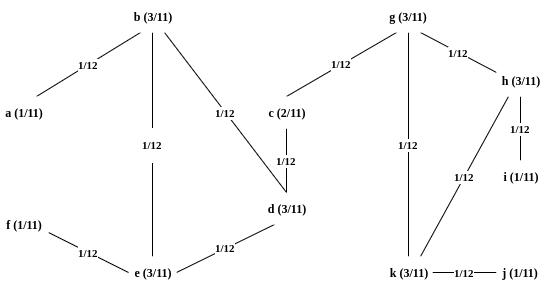
\includegraphics[width=0.8\textwidth]{k-path-initial-weights}
	\caption{Example of assignment of normalized degrees and initial edge weights \cite{ref-35}.}
	\label{fig:initial-edge-weight-graph}
\end{figure}

\subsubsection*{\textit{Simulation of message propagation through random simple $\mathcal{K}$-paths}}
In the second step authors of \cite{ref-35} has introduced $\rho$ simple random walks of length at most $\mathcal{K}$ on the network. The ERW-$\mathcal{K}$-path algorithm performs the following operations at each iteration.
\begin{enumerate}
	\item A node $v_n \in V$ of the graph $G$ is selected according to one of the following two possible strategies:
	\begin{enumerate}[label=\alph*.]
		\item uniformly at random, with a probability:
		\begin{equation}
		P(v_n) = \dfrac{1}{\mid V \mid}
		\end{equation}
		\item with a probability proportional to its normalized degree $\delta(v_n)$, given by:
		\begin{equation}\label{probability-of-normalized-degree}
		P(v_n) = \dfrac{\delta(v_n)}{\sum_{v_k \in V} \delta(v_k)}
		\end{equation}
	\end{enumerate}
	\item All the edges in $G$ are marked as not traversed
	\item The procedure \textit{MessagePropagation} is invoked
\end{enumerate}
\textbf{\textit{MessagePropagation:}}\\
This very procedure carries out a loop as long as \textit{both} the following conditions hold true:
\begin{itemize}
	\item The length of the path currently generated is no greater than $k$. This is managed through a length counter $N$
	\item Assuming that the walk has reached the node $v_n$, there must exist at least an incident edge on $v_n$ which has not been already traversed. To do so, a flag $T(e_m)$ is attached to each edge $e_m \in E$, such that
	\begin{equation}
	T(e_m) = \begin{cases}
	1 & \text{if $e_m$ has already been traversed}\\
	0 & \text{otherwise}
	\end{cases} 
	\end{equation}
	the following condition must hold true:
	\begin{equation}
	\mid I(v_n) \mid \quad > \sum\limits_{e_k \in I(v_n)} T(e_k)
	\end{equation}
	being $I(v_n)$ the set of edges incident onto $v_n$.
\end{itemize}
If the conditions above are satisfied, the \textit{MessagePropagation} procedure selects an edge $e_m$ by applying two strategies:
\begin{enumerate}[label=\alph*.]
	\item uniformly at random, with probability
	\begin{equation}
	P(e_m) = \dfrac{1}{\mid I(v_n) \mid - \sum\limits_{e_k \in I(v_n)} T(e_k)}
	\end{equation}
	among all the edges $e_m \in \left\{ I(v_n) | T(e_m) = 0\right\}$ incident on $v_n$ (i.e., excluding already traversed edges)
	\item with a probability proportional to the edge weight $\omega_l (e_m)$, given by
	\begin{equation}\label{probability-edge-weight}
	P(e_m) = \dfrac{\omega_l (e_m)}{\sum\limits_{e_m \in \hat{I}(v_n)} \omega_l (e_m)}
	\end{equation}
	being $\hat{I}(v_n) = \{e_k \in I(v_n) | T(e_k) = 0\}$ and $\omega_l (e_m) = \omega_{l-1} (e_m) + \beta \cdot T(e_m)$ if $1 \le l \le k\rho$
\end{enumerate}
Let $e_m$ be the selected edge and let $v_{n+1}$ be the node reached from $v_n$ by means of $e_m$. The \textit{MessagePropagation} procedure awards a bonus $\beta$ to $e_m$, sets $T(e_m) = 1$ and increases the counter $N$ by 1. The message propagation activity continues from $v_{n+1}$.

\begin{algorithm}[ht!]
	\caption{WERW-$\mathcal{K}path$(Graph $G = \langle V, E\rangle$, int $k$, int $\rho$, float $\beta$)}
	\label{algo:werw-kapth-algorithm}
	\SetAlgoLined
	\DontPrintSemicolon
	Assign each node $v_n \in V$ its normalized degree\;
	Assign each edge $e_m \in E$ the uniform probability function as weight\;
	\For{$i=1$ to $\rho$}{
		$N \gets 0$ a counter to check the length of the $k$-path\;
		$v_n \gets $ a node chosen uniformly at random in $V$\;
		MessagePropagation($v_n$, $N$, $k$, $\beta$)
	}
\end{algorithm}
\begin{algorithm}[ht!]
	\caption{MessagePropagation(Node $v_n$, int $N$, int $k$, float $\beta$)}
	\label{algo:message-propagation-algorithm}
	\SetAlgoLined
	\DontPrintSemicolon
	\While{$N < k$ and $\left[ \mid I(v) \mid > \sum_{e \in I(v)} T(e)\right]$}{
		$e_m \gets e_m \in \left\{I(v) | T(e_m) = 0\right\}$, chosen uniformly at random\;
		Let $v_{n+1}$ be the node reached by $v_n$ through $e_m$\;
		$\omega (e_m) \gets \omega (e_m) + \beta$\;
		$T(e_m) \gets 1$\;
		$v_n \gets v_{n+1}$\;
		$N \gets N + 1$\; 
	}
\end{algorithm}
Algorithm (\ref{algo:werw-kapth-algorithm}) and algorithm (\ref{algo:message-propagation-algorithm}) described in this section adopts uniform probability distribution functions in order to choose nodes and edges purely at random and as discussed before it is called ERW-$\mathcal{K}$path. Although, a weighted version of the same algorithm, called WERW-$\mathcal{K}$path, both algorithms would differ only in line 5,  adopting weighted functions specified in Equations (\ref{probability-of-normalized-degree}) and (\ref{probability-edge-weight}).

The time complexity if the ERW-$\mathcal{K}$Path algorithm is $\mathcal{O}(\kappa \rho)$. If, $\rho = \mid E \mid - 1$, then algorithm achieves a good tradeoff between accuracy and computational costs. In fact, in such a case, the worst case time complexity of ERW-$\mathcal{K}$Path algorithm is $\mathcal{O}(\kappa \mid E \mid)$.

\subsubsection*{Fast $\mathcal{K}$-Path Community Detection}
In \cite{ref-28}, Meo et al. introduced a generalized LM \cite{ref-27} that outperforms other community detection techniques and also slightly improves results of the original LM. Authors of \cite{ref-28} named their proposed algorithm as \textit{Fast $\mathcal{K}$-Path Community Detection} (or shortly, FKCD), hence-forth FKCD. This particular algorithm inhabits the main features of the original LM and relies on three steps:\\\\
\textit{(i)} Ranking edges by using the WERW-$\mathcal{K}$path algorithm\\
\textit{(ii)} Calculating the proximity (the inverse of the distance) between each pair of connected nodes\\
\textit{(iii)} Partitioning the network into communities so to optimize the network modularity \cite{ref-1}

\subsubsection*{Ranking Edges by Using WERW-$\mathcal{K}$path}
FKCD algorithm requires a ranking criterion to compute the aptitude of all the edges to propagate information through the network. To do so, FKCD invokes the WERW-$\mathcal{K}$path algorithm (\ref{sec:k-path-edge-centrality}). Once all the edges have been labeled with their $\mathcal{K}$-path edge centrality, a ranking in decreasing order of centrality could be obtained. The computational cost of this step is $\mathcal{O} (\kappa \mid E \mid)$, with $k$ length of the $\mathcal{K}$-paths and $\mid E \mid$ cardinality of $E$.

\subsubsection*{Calculation of Proximity Between Each Pair of Connected Nodes}
In the second step, FKCD calculates the proximity of each connected pair of nodes using a $L_2$ distance, commonly known as \textit{Euclidean distance} which has been discussed briefly in this thesis in section (\ref{vertexsimilarity}). $L_2$ distance for FKCD is calculated as:
\begin{equation}\label{eq:node-proximity}
r_{ij} = \sqrt{\sum_{\kappa = 1}^{n} \dfrac{(L^\kappa (e_{i \kappa}) - L^\kappa (e_{\kappa j}))^2}{d(\kappa)}}
\end{equation}
where $L^\kappa(e_{i \kappa})$ (resp., $L^\kappa(e_{\kappa j})$) is the $kappa$-path edge-centrality of the edge $e_{i \kappa}$ (resp., $e_{\kappa j}$) and $d(\kappa)$ is the degree of the node.

Even though $L_2$ measure would return a distance, in this case, the higher $L^\kappa (e_{i \kappa})$ (resp., $L^\kappa (e_{\kappa j})$), the more the nodes are near, instead of distance. This step of FKCD algorithm is theoretically computationally expensive because it should require $\mathcal{O} (\mid V \mid^2)$ iterations. But in practice, by adopting optimization techniques, its near-linear computation cost is $\mathcal{O} (\bar{d}(v) \mid V \mid)$, where $\bar{d}(v)$ is the mean degree of all the nodes of the network (it's usually small in very large networks) \cite{ref-28}.

\subsubsection*{Network Partitioning}\label{subsec:network-partitioning}
The principal idea of network partitioning is inspired by the LM \cite{ref-27} for detecting the community structure of weighted networks in a near linear time. Network partitioning is an iterative process. At each iteration FKCD repeats two simple steps:\\\\
\textit{(i)} Each node is assigned to a community chosen in order to maximize the network modularity $Q$. This process has been discussed explicitly in section (\ref{sebsec:modularity-optimization}).\\
\textit{(ii)} The second step produces a \textit{meta-network} whose nodes are those communities previously found.
partitioning ends when no further improvements of $Q$ can be obtained.

For this third step, cost of computation is $\mathcal{O} (\gamma \mid V \mid)$, where $\mid V \mid$ is the cardinality of $V$ and $\gamma$ is the number of iterations required by the algorithm to converge (usually, $\gamma < 5$) \cite{ref-28}.

\begin{algorithm}
	\caption{FKCD(Graph $G = (V, E)$, int $\kappa$)}
	\label{algo:fkcd-algorithm}
	\SetAlgoLined
	\DontPrintSemicolon
	WERW-Kpath(G, $\kappa$)\tcp*{Using algorithm (\ref{algo:werw-kapth-algorithm})}
	CalculateDistance(G)\tcp*{Calculates distance with Eq. (\ref{eq:node-proximity})}
	\While{$Q$ increases at least of $\in$ (arbitrarily small)}{
		$P = $ Partition(G)\tcp*{Partitioning is done with (\ref{subsec:network-partitioning})}
		$Q \gets $ NetworkModularity(P)\tcp*{Measures modularity with Eq. (\ref{sumoverclusters})}
	}
\end{algorithm}
The computational cost for the whole strategy described in this algorithm is near linear. In fact, $\mathcal{O} (\kappa \mid E \mid + \;\bar{d} (e) \mid V \mid + \;\gamma \mid V \mid) = \mathcal{O} (\tau \mid E \mid)$, by adopting efficient graph memorization in order to minimize the execution time for the computation of Equations (\ref{sumoverclusters}) and (\ref{eq:node-proximity}).

\vfill
\pagebreak

% ================================================================================================= %

\subsection{Girvan-Newman Algorithm Architecture}
\textit{Edge betweenness} is the number of shortest paths between all vertex pairs that run along the edge. It is an extension to edges of the popular concept of site betweenness, introduced by Freeman \cite{ref-11} and expresses the importance of edges in processes like information spreading, where information usually spreads through the shortest paths. It is intuitive that inter-community edges have a large value of the edge betweenness, because many \textit{shortest paths} connecting vertices of different communities will pass through them (\ref{edgebetweenness}). If there are two or more geodesic paths with the same endpoints that run through an edge, the contribution of each of them to the betweenness of the edge must be divided by the multiplicity of the paths. The betweenness of all edges of the graph can be calculated in a time that scales as $\mathcal{O}(mn)$, or $\mathcal{O}(n^2)$ on a sparse graph, with techniques based on breadth-first-search \cite{ref-12}.

In the context of information spreading, it is very common and realistic that signals flow across random rather than geodesic paths. In this case, the betweenness of an edge is given by the frequency of the passages across the edge of a random walker running on the graph (random-walk betweenness). A random walker moving from a vertex follows each adjacent edge with equal probability. A pair of vertices is chosen at random, $s$ and $t$. The walker starts at $s$ and keeps moving until it hits $t$, where it stops. Calculation of random-walk betweenness requires the inversion of an $n \times n$ matrix (once), followed by obtaining and averaging the flows for all pairs of nodes. The first task requires a time $\mathcal{O}(n^3)$, the second $\mathcal{O}(mn^2)$, for a total complexity $\mathcal{O}[(m + n)n^2]$, or $\mathcal{O}(n^3)$ for a sparse matrix. The complete calculation requires a time of $\mathcal{O}(n^3)$ on a sparse graph.

Current-flow betweenness is defined by considering the graph a resistor network, which edges having unit resistance. If a voltage difference is applied between two vertices, each edge carries some amount of current, that can be calculated by solving \textit{Kirchoff's equations}. The procedure is repeated for all possible vertex pairs. The calculation of current-flow betweenness has the same complexity as random-walk betweenness $\mathcal{O}[(m + n)n^2]$, or $\mathcal{O}(n^3)$ for a sparse graph.

\subsubsection*{Betweenness Centrality}\label{betweennesscentrality}
Girvan-Newman algorithm uses \textit{betweenness centrality} to detect community structure in a graph. To sidestep the shortcomings of the hierarchical clustering method, in this algorithm, they proposed an alternative approach. Instead of trying to construct a measure that tells which edges are most central to communities, in this algorithm they focused on this edges that are least ``central", the edges that are most ``between" communities. The betweenness centrality of a vertex $v$ is defined as the number of shortest paths between pairs of other vertices that run though $v$ \cite{ref-11}. 
\begin{equation}
C_B(v) = \sum\limits_{s \neq v \neq t \in V} \dfrac{\sigma_{st}(v)}{\sigma_{st}}
\end{equation}
where $\sigma_{st}$ denotes the number of shortest paths from $s \; \in \; V$ to $t \; \in \; V$ and $\sigma_{st}(v)$ denotes the number of shortest paths from $s$ to $t$ that some $v \; \in \; V$ lies on. 

The betweenness centrality of a node scales with the number of pairs of nodes as implied by the summation indices. Therefore, the calculation may be re-scaled by dividing through by the number of pairs of nodes not including $v$, so that $C_B(v) \; \epsilon \; [0,1]$.

For \textit{undirected} networks, the normalized betweenness centrality is given by
\begin{equation}
C_B(v) = \dfrac{2}{n^2 - 3n + 2} \cdot \sum\limits_{s \neq v \neq t \in V} \dfrac{\sigma_{st}(v)}{\sigma_{st}}
\end{equation}
For \textit{undirected} networks, we divided the betweenness centrality by $(n - 1)(n - 2) / 2$, where $n$ is the number of nodes in the graph.

For \textit{directed} networks, the normalized betweenness centrality is given by
\begin{equation}
C_B(v) = \dfrac{1}{n^2 - 3n + 2} \cdot \sum\limits_{s \neq v \neq t \in V} \dfrac{\sigma_{st}(v)}{\sigma_{st}}
\end{equation}
For \textit{directed} networks, we divided the betweenness centrality by $(n - 1)(n - 2)$, where $n$ is the number of nodes in the graph \cite{ref-17}.

Usually, values are normalized to obtain values between 0 and 1. The highest possible value occurs when one node is located on every single shortest path (\textit{star graph}). An example from \cite{ref-17}, let's consider the following undirected network:

\begin{figure}[H]
	\centering
	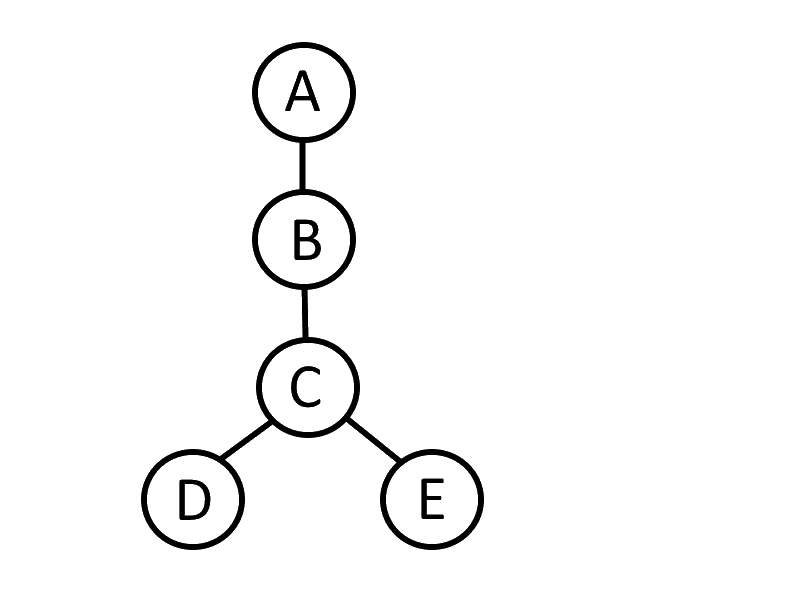
\includegraphics[width=0.4\textwidth]{betweenness_graph.png}
	\caption{A simple undirected network}
	\label{betweenness_graph}
\end{figure}

\begin{table}[!h]
	\centering
	\begin{tabular}{|c | c | c |}
		\cline{2-3}\multicolumn{1}{c|}{} 
		& 		$C_{B}(v)$	& $Normalized \; C_{B}(v)$ \\\hline 
		$A$		& 0 		& 0 						\\\hline 
		$B$ 	& 3.0		& 0.5 						\\\hline 
		$C$ 	& 5.0		& 0.8$\overline{3}$ 		\\\hline 
		$D$ 	& 0 		& 0							\\\hline 
		$E$ 	& 0 		& 0 						\\\hline 
	\end{tabular}
	\caption{An example of betweenness centrality measure calculated from Figure (\ref{betweenness_graph})}
\end{table}

Girvan-Newman algorithm calculates the betweenness using the fast algorithm of Newman \cite{ref-1, ref-13}. This calculates the betweenness for $m$ edges in a graph of $n$ vertices in time $\mathcal{O}(mn)$. To reduce the running time of the algorithm further, one might be tempted to calculate the betweenness of all the edges only once and then remove them in order of decreasing betweenness. But this strategy does not work well because if two communities are connected by more than one edge, then there is no guarantee that all of those edges will have high betweenness. In practical applications, the Girvan-Newman algorithm with betweenness centrality gives better results than adopting other centrality measures \cite{ref-12}, although Girvan-Newman algorithm cannot find overlapping communities, as each vertex is assigned to a single cluster.

\subsubsection*{Fast Algorithm of Newman}\label{sub:fastalgorithm}
To detect community structure in a sparse network faster, Newman has proposed an algorithm, known as \textit{Fast algorithm of Newman}. This algorithm is based on the idea of modularity. Given any network, the GN community structure algorithm \cite{ref-1} always produces some division of the vertices into communities, regardless of whether the network has any natural such division \cite{ref-13}. To test whether a particular division is meaningful, this algorithm defines a quality function or\textit{ modularity $Q$} as follows \cite{ref-1}.

Let $e_{ij}$ be one-half of the fraction of edges in the network that connect vertices in group $i$ to those in group $j$, so that the total fraction of such edges is $e_{ij} + e_{ji}$. The only exception will be the diagonal elements $e_{ii}$, which are equal to the fraction of edges that fall within group $i$ (with no factor of a half). Then $\sum_i e_{ii}$ is the total friction of edges that fall within groups. All other edges fall between groups. The maximum value of this sum is 1, and  a division of the network into communities is good if this quality is large, meaning it is of order 1.

Let $a_i$ be the fraction of all ends that are attached to vertices in group $i$. We can calculate $a_i$ straightforwardly by noting that $a_i = \sum_j e_{ij}$. If the ends of edges are connected together at random, the fraction of the resulting edges that connect vertices within group $i$ is $a_i^2$. We define the modularity $Q$ as:
\begin{equation}
Q = \sum\limits_i (e_{ii} - a_i^2)
\end{equation}

If a particular division gives no more within-community edges than would be expected by random chance, this modularity is $Q = 0$. Values other than 0 indicates deviations from randomness and in practice values greater than about 0.3 appear to indicate significant community structure \cite{ref-12}.

The fast algorithm of Newman starts with a state in which each vertex is a sole member of one of $n$ communities, it repeatedly joins communities together in pairs, choosing at each step the  join that results in the greatest increase (or smallest decrease) in $Q$. The process of this algorithm can be represented as a dendrogram as in Figure(\ref{dendrogram}). Since, the joining of a pair of communities between which there are no edges at all can never result in an increase in $Q$, the algorithm only considers those pairs between which there are edges, of which there will at any time be at most $m$, where $m$ is the number of edges in the graph. The change in $Q$ upon joining two communities is given by
\begin{equation}
\Delta Q = e_{ij} + e_{ji} - 2 a_i a_j = 2(e_{ij} - a_ia_j)
\end{equation}
which can clearly be calculated in constant time. There is a maximum of $n - 1$ join operations necessary to construct the complete dendrogram and hence the entire algorithm runs in time $\mathcal{O}((m + n)n)$, or $\mathcal{O}(n^2)$ on a sparse graph \cite{ref-13}.

% ================================================================================================== %

\subsection{Modularity Maximization Technique}\label{subsec:modularity_maximization}
A \textit{quality function} is a function that assigns a number to each partition of a graph. In this way, one can rank partitions based on their score given by the quality function. Partition with high scores are marked as ``good", so the one with largest score is by definition the best. Nevertheless, one should keep in mind that the question is when a partition is better than another one is ill-posed, and the answer depends on the specific concept of community and/or quality function adopted.

A quality function $Q$ is additive if there is an elementary function $q$ such that, for any partition $\mathcal{P}$ of a graph
\begin{equation}\label{quality-eq-1}
Q(\mathcal{P}) = \sum\limits_{\mathcal{C} \in \mathcal{P}} q(\mathcal{C}),
\end{equation}
where $\mathcal{C}$ is a generic cluster of partition $\mathcal{P}$. Above Eq.(\ref{quality-eq-1}) states that the quality of a partition is given by the sum of the qualities of the individual clusters. The function $q(\mathcal{C})$ could be any of the cluster fitness functions adopted.

An example of a quality function is the performance $P$, which counts the number of correctly "interpreted" pairs of vertices, i.e. two vertices belonging to the same community and connected by an edge, or two vertices belonging to different communities and not connected by an edge. The definition of performance, for a partition $\mathcal{P}$, is
\begin{equation}
P(\mathcal{P}) = \frac{\vert \{(i,j) \in E, C_i = C_j\} \vert + \vert (i,j) \notin E, C_i \neq C_j\vert}{n(n-1)/2}
\end{equation}
By definition, $0 \; \le \; P(\mathcal{P}) \; \le \; 1$ \cite{ref-6}. 

Modularity is the fraction of the edges that fall within the given groups minus the expected fraction if edged were distributed at random. the value of modularity lies in the range of $[-1/2,1)$. It is positive if the number of edges within groups exceeds the number of expected on the basis of change. For a given division of the network's vertices into some modules, modularity reflects the connection of edges within modules compared with the random distribution of links between all nodes regardless of modules. In the most common version of this concept, randomization of the edges is done so as to preserve the degree of each vertex.

Consider a graph with $n$ nodes and $m$ edges such that the graph can be partitioned into two communities using a membership variable $s$. If a node $i$ belongs to community $X$, $s_i = 1$, or if $i$ belongs to community $Y$, $s_i = -1$. Let the adjacency matrix of the network be presented by $\textbf{A}$, where $\textbf{A}_{ij} = 0$ means that there's no edge between node $i$ and $j$. On the other hand, $\textbf{A}_{ij} = 1$ means there is an edge between the two. Also for simplicity, we consider an undirected graph. Thus, $\textbf{A}_{ij} = \textbf{A}_{ji}$ \footnote{It is important to note that multiple edges may exist between two nodes, but here we asses the simplest case.}. Modularity $Q$ is then defined as the fraction of  edges that fall within group $X$ or $Y$, minus the expected number of edges within groups $X$ and $Y$ for a random graph with the same node degree distribution as the given network.

The expected number of edges shall be computed using the concept of configuration models \cite{ref-16}. The configuration model is a randomized realization of a particular network. Given a network with $n$ nodes, where each node $i$ has a node degree $k_i$, the configuration model cuts each edge into two halves, and then each half edge called a \textit{stub}, is rewired randomly with any other \textit{stub} in the network even allowing self-loops. Thus, even though the node degree distribution of the graph remains intact, the configuration model results in a completely random graph.

Let the total number of \textit{stubs} be $l_n$:

\begin{equation}
l_n = \sum\limits_i k_i = 2m
\end{equation}

Now, if we randomly select two nodes $i$ and $j$ with node degrees $k_i$ and $k_j$ respectively and rewire the stubs for these two nodes, then:
\newline\newline
\textbf{Expectation of full edges between $i$ and $j$ =$\dfrac{(Full \; edges \; between \; i \; and \; j )}{(Total \; number \; of \; rewiring \; possibilities)}$} 
\newline\newline
The total number of rewiring possible is equal to the number of \textit{stubs} remaining after choosing a particular \textit{stub}, $l_{n-1}$. For large values on $n$, $l_{n-1} \approx l_n$. Thus,
\newline\newline
\textbf{Expected number of full edges between $i$ and $j$ = $\dfrac{k_i k_j}{l_n}$}
\newline\newline

Hence, the difference between the actual number of edges between node $i$ and $j$ and the expected number of edges between them is:

\begin{center}
	$\textbf{A}_{ij} - \frac{k_i k_j}{2m}$
\end{center}

Summing over all node pairs gives the equation for modularity, $\textbf{Q}$.
\begin{equation}\label{modularity_Q}
Q = \dfrac{1}{2m} \sum\limits_{ij}\left[\textbf{A}_{ij} - \dfrac{k_i k_j}{2m}\right] \dfrac{s_i s_j + 1}{2}
\end{equation}

It is important to note that Eq.(\ref{modularity_Q}) holds good for partitioning into two communities only. Hierarchical\footnote{Partitioning into two communities, then two sub-communities further partitioned into two smaller sub-communities only to maximize \textbf{Q}.} partitioning is a possible approach to identify multiple communities in a network. Additionally, Eq.(\ref{modularity_Q}) can be generalized for partitioning a network into $n_c$ communities.
\begin{equation}
Q = \dfrac{1}{(2m)} \sum\limits_{ij}\left[\textbf{A}_{ij} - \dfrac{k_i k_j}{(2m)}\right] \delta(C_i, C_j)
\end{equation}
Where $A_ij$ represents the weight of the edge between $i$ and $j$, $k_i = \sum_j A_ij$ is the sum of the weights of the edges attached to vertex $i$, $C_i$ is the community to which vertex $i$ is assigned, the $\delta$-function $\delta(u,v)$ is 1 if $u = v$ and 0 otherwise and $m = \frac{1}{2} \sum_{ij}A_{ij}$ \cite{ref-27}.
 
Since the only contributions to the sum come from vertex pairs belonging to the same cluster, we can group these contributions together and rewrite the sum over the vertex pairs as a sum over the clusters,
\begin{equation}\label{sumoverclusters}
Q = \sum\limits_{c=1}^{n_c} \left[ \dfrac{l_c}{m} - \left( \dfrac{d_c}{2m}\right)^2\right]
\end{equation}
Here, $n_c$ is the number of clusters, $l_c$ the total number of edges joining vertices of module $c$ and $d_c$ the sum of the degrees of the vertices of $c$. In Eq.(\ref{sumoverclusters}), the first term of each sum and is the fraction of edges of the graph inside the module, whereas the second term represents the expected fraction of edges that would be there if the graph were a random graph with same expected degree of each vertex.

A nice feature of modularity is that it can be equivalently expressed both in terms of the intra-cluster edges, as in Eq.(\ref{sumoverclusters}), and in terms of the inter-cluster edges. In fact, the maximum of modularity can be expressed as:
\begin{equation}\label{modularity_Q_max}
\begin{array}{c c lc}
Q_{max} & = & \max\limits_{\mathcal{P}} \left\lbrace \sum\limits_{c=1}^{n_{c}}\left[\frac{l_{c}}{m} - \left(\frac{d_{c}}{2m}\right)^2\right]\right\rbrace \\
& = & \frac{1}{m}\max\limits_{\mathcal{P}} \left\lbrace \sum\limits_{c=1}^{n_{c}}\left[l_{c} - Ex(l_{c})\right] \right\rbrace \\
& = & - \frac{1}{m}\min\limits_{\mathcal{P}} \left\lbrace - \sum\limits_{c=1}^{n_{c}}\left[l_{c} - Ex(l_{c})\right] \right\rbrace,
\end{array}
\end{equation}
where $\max_{\mathcal{P}}$ and $\min_{\mathcal{P}}$ indicate the maximum and the minimum overall possible graph partitions $\mathcal{P}$ and Ex($l_c$) = $d_c^2/4m$ indicates the expected number of links in the cluster $c$ in the null model of modularity. By adding and subtracting the total number of edges $m$ of the graph one finally gets
\begin{equation}\label{modularity_Q_max_cut}
\begin{array}{c c lc}
Q_{max} & = & -\dfrac{1}{m} \min\limits_{\mathcal{P}}\left\lbrace \left[ \left( m - \sum\limits_{c=1}^{n_c} l_c\right) - \left( m - \sum\limits_{c=1}^{n_c} Ex(l_c)\right) \right] \right \rbrace \\
& = & - \frac{1}{m} \min\limits_{\mathcal{P}} (\vert Cut_{\mathcal{P}} \vert - ExCut_{\mathcal{P}}).
\end{array}
\end{equation}
In the last expression $\vert Cut_{\mathcal{P}} \vert = m - \sum_{c=1}^{n_c} l_c$ is the number of inter-cluster edges of partition $\mathcal{P}$, and $ExCut_{\mathcal{P}} = m - \sum_{c=1}^{n_c} Ex(l_c)$ is expected number of inter-cluster edges of the partition in modularity's null model.

\subsubsection*{Modularity Optimization }\label{sebsec:modularity-optimization}
Modularity is by far the most used and best-known quality function \cite{ref-6}. By assumption, a high value of modularity indicates good partitions. So, the partition corresponding to its maximum value on a given graph might be the best or at least a very good one. An exhaustive optimization of $Q$ is not possible, due to the huge number of ways in which it is possible to partition a graph, even when the latter is small. Besides, the true maximum is out of reach, as it has been recently proved that modularity is an NP-complete problem \cite{ref-18}, so it is probably impossible to find the solution in a time growing polynomially with the size of the graph. However, there are currently several algorithms able to find fairly good approximations of the modularity maximum in a reasonable time.


\subsection{Hierarchical Clustering}\label{sub:hierarchicalclustering}
The starting point of any \textit{hierarchical clustering} method is the definition of a similarity measure between vertices. After the measure is chosen, it computes the similarity for each pair of vertices, no matter if they are connected or not \cite{ref-6}. At the end of this process, a new $ n \times n$ matrix $X$, the \textit{similarity matrix} is produced. hierarchical clustering techniques aim at identifying groups of vertices with high similarity and can be classified into two categories:

\begin{enumerate}
	\item \textit{Agglomerative algorithms}, in which clusters are iteratively merged if their similarity is sufficiently high
	\item \textit{Divisive algorithms}, in which clusters are iteratively split by removing edges connecting vertices with low similarity
\end{enumerate}

For the scope of this section we will focus on agglomerative algorithms. This thesis will also get into Divisive algorithms as it proceeds through different other methods in a later stage. Agglomerative algorithms are bottom-up, as one starts from the vertices as separate clusters (singletons) and ends up with the graph as a unique cluster. Science clusters are merged based on their mutual similarity. It is essential to define a measure that estimates how similar clusters are out of the matrix $X$. In \textit{single-linkage clustering}, the similarity between the two groups is the minimum element $x_{ij}$, with $i$ in one group and $j$ in the other.

This whole procedure can be better illustrated with the help of \textit{dendrogram} which is a very common way to represent the hierarchical structure of graph is to draw a dendrogram, like the one in Figure (\ref{dendrogram}).

\begin{figure}[H]
	\centering
	\begin{minipage}[b]{0.5\textwidth}
		\centering
		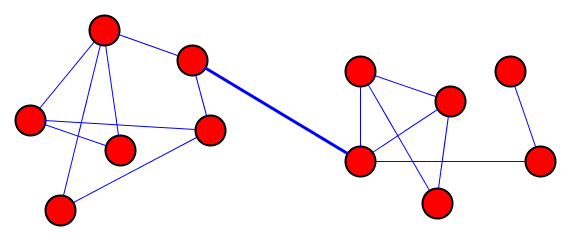
\includegraphics[width=\textwidth]{edge_betweenness.png}
		\caption{An example of edge betweenness}
		\label{edgebetweenness}
	\end{minipage}
	\begin{minipage}[b]{0.45\textwidth}
		\centering
		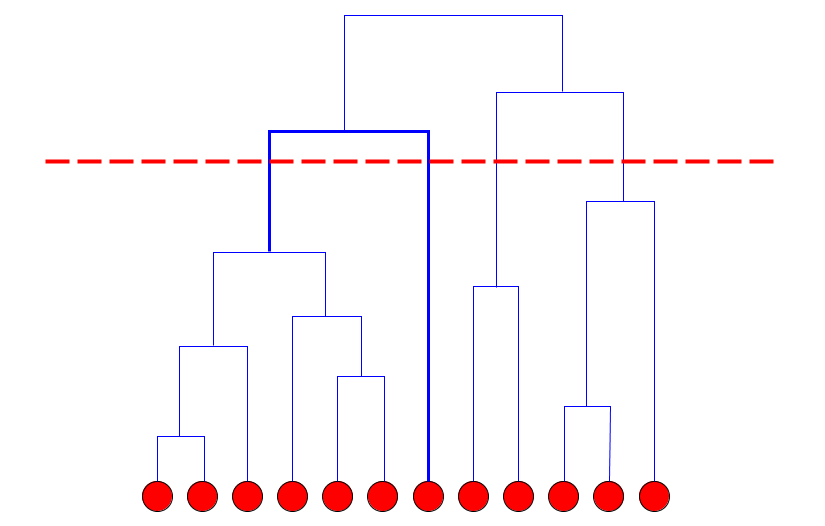
\includegraphics[width=\textwidth]{dendrogram.png}
		\caption{A dendrogram with twelve nodes from the graph in Figure (\ref{edgebetweenness})}
		\label{dendrogram}
	\end{minipage}
\end{figure}

Here, partitions of a graph with twelve vertices are shown. At the bottom, each vertex is its own module (the \textit{leaves} of the tree). By moving upwards, groups of vertices are successively aggregated. Based on the  given similarity measures \textit{mergers} of communities are represented by horizontal lines. The uppermost level represents the whole graph as a single community. Cutting the diagram horizontally at some height, as shown in the Figure (dashed line), displays one partition of the graph. The diagram is hierarchical by construction: each community belonging to a level is fully included in a community at a higher level.

Hierarchical clustering has the advantage that it does not require any preliminary knowledge on the number and size of the clusters. The result depends on the specific similarity measure adopted as described in section (\ref{vertexsimilarity}). Another problem is that vertices with just one neighbor are often classified as a separated cluster, which does not make any sense. The major weakness of agglomerative hierarchical clustering is that it does not scale well \cite{ref-6}. If points of a graph are embedded in space, so that the distance can be used as a dissimilarity measure as described in section (\ref{vertexsimilarity}), the computational complexity is $\mathcal{O}(n^2)$ for single linkage, $\mathcal{O}(n^2 \log n)$ for the complete and average linkage schemes. For graph clustering, where distance is not trivially defined, the complexity can become much heavier if the calculation of the chosen similarity measure is costly.

\subsubsection*{Vertex Similarity}\label{vertexsimilarity}
It is natural to assume that communities are groups of vertices similar to each other. The similarity between each pair of vertices with respect to some reference property, local or global, no matter whether they are connected by an edge or not can be computed. Each vertex ends up in the cluster whose vertices are most similar to it.

If it were possible to embed the graph vertices in an $n$-dimensional \textit{Euclidean space}, by assigning a position to them, one could use the \textit{distance} between a pair of vertices as a measure of their similarity \footnote{It is actually a measure of dissimilarity because similar vertices are expected to be close to each other.}. Given the two data points $A = (a_1, a_2, \dots, a_n)$ and $B = (b_1, b_2, \dots , b_n)$, one could use any norm $L_m$.\newline \newline
The \textit{Euclidean distance}($L_2$-norm):
\begin{equation}
d_{AB}^E = \sum_{k=1}^{n} \sqrt{(a_k - b_k)^2}
\end{equation}
the \textit{Manhattan distance}($L_1$-norm)
\begin{equation}
d_{AB}^M = \sum_{k=1}^{n} \vert a_k - b_k \vert
\end{equation}
and the $L_\infty$-norm will be
\begin{equation}
d_{AB}^\infty = \underset{k \in [1,n]}{\max} \vert a_k - b_k \vert
\end{equation}

Another popular spatial measure is the \textit{cosine similarity}, defined as
\begin{equation}\label{eq:cosine_similarity}
\rho_{AB} = \arccos \dfrac{\textbf{a} \cdot \textbf{b}}{\sqrt{\sum\limits_{k=1}^{n}{a_k^2}} \sqrt{\sum\limits_{k=1}^{n}{b_k^2}}}
\end{equation}
where $\textbf{a}\cdot\textbf{b}$ is the dot product of vectors \textbf{a} and \textbf{b}. The variable $\rho_{AB}$ is defined in the range $[0,\pi)$.

If the graph cannot be embedded in space, the similarity must be necessarily inferred from adjacency relationships between vertices or node properties. A possibility is to define a distance between vertices like \cite{ref-8, ref-9}.
\begin{equation}
d_{ij} = \sqrt{\sum_{k \neq {i,j}} (\textbf{A}_{ik} - \textbf{A}_{jk})^2}
\end{equation}
where \textbf{A} is the adjacency matrix. This is a dissimilarity measure, based on the concept of structural equivalence \cite{ref-10}. Two vertices are structurally equivalent if they have the same neighbors, even if they are not adjacent themselves. If $i$ and $j$ are structurally equivalent, $d_{ij} = 0$. Vertices with a large degree and different neighbors are considered very \textit{far} from each other. Alternatively, one could measure the \textit{overlap} between the neighborhoods $\varGamma(i)$ and $\varGamma(j)$ of vertices $i$ and $j$, given by the ratio between the intersection and the union of the neighborhoods, i.e.
\begin{equation}\label{eq:neihborhood-overlap}
\omega_{ij} = \dfrac{\vert \varGamma(i) \cap \varGamma(j) \vert}{\vert \varGamma(i) \cup \varGamma(j) \vert}
\end{equation}

Another very widely used measure related to structural equivalence is the \textbf{\textit{Pearson Correlation}} between columns and rows of the adjacency matrix,
\begin{equation}
C_{ij} = \dfrac{\sum\limits_{k} (A_{ik} - \mu_i) (A_{jk} - \mu_j)}{n \sigma_i \sigma_j}
\end{equation}
where the averages $\mu_i = (\sum\limits_j A_{ij} / n)$ and the variances $\sigma_i = \sqrt{\sum\limits_j (A_{ij} - \mu_i)^2} / n$

\section{Dynamic Community Detection Algorithms}\label{sec:dynamic_community_algorithms}
In section (\ref{subsub:dynamic_community}), dynamic community detection and its life cycle is described in brief. Difficulty in accessing time-stamped data for real systems represented in a graph was the main problem for dynamic community detection and observation. Until recently, availability of time-stamped graph data representing real systems lead to a path of community detection and observation, enabling to monitor the evolution of communities in time. Figure (\ref{fig:community_evolution}) illustrates the different scenarios of the community life-cycle.

The first study about community detection and observation was carried out by Hopcroft et al. in  \cite{ref-52} in 2004. Authors in this article analyzed snapshots of the citation graph data from NEC CiteSeer Database. These snapshots covered the period from 1990 to 2001. In that article, author used \textit{hierarchical clustering} (section \ref{sub:hierarchicalclustering}) to detect communities, where similarity between vertices (nodes) is the \textit{cosine similarity} (Equation \ref{eq:cosine_similarity}) of the vectors describing the corresponding papers. Authors found the best matching communities across different snapshots and in this way they were able to observe the evolution of community structures.

In 2007, Palla et al. in \cite{ref-23} performed a semantic analysis of dynamic communities. The authors used two different data-sets from two different systems. One was a year's phone call data and another one was a graph of the collaboration network between scientists, describing co-authorship of papers over 142 months. They faced a few challenges along the way to determine the best course of action to detect and observe communities over time, the first challenge was to identify the image of community $\mathcal{C}(t+1)$ at time $t+1$ among the communities of the graph at time $t$. A simple way to see the evolution of community is to see the overlap of communities between time $t$ and $t+1$. The problem is at time-stamp $t+1$, a community that existed at time-stamp $t$ might have changed and in this process, it might miss the actual evolution of the communities. Authors of \cite{ref-23}, solved the problem by using Clique Percolation Method (see \cite{ref-6} section 11.1). The general idea is to analyze a graph $\mathcal{G}(t, t+1)$, obtained by merging two snapshots $\mathcal{G}(t)$ and $\mathcal{G}(t+1)$ of evolving graph at time-stamp $t$ and $t+1$. So these, CPM communities {$\mathcal{C}^{t+1}$} has the largest relative overlap with community {$\mathcal{C}^t$} at time $t$.

Sun et al. in \cite{ref-53}, used a method of information compression called MDL (Minimum Description Length) described in \cite{ref-54} to find the minimum encoding cost for the description of a time sequence of graphs and their partitions in communities. In this method, a bipartite graph is considered and the time sequence of the graphs can be separated into segments. For each graph segment, it is possible to define encoding cost, which combines the encoding cost of the partition of the graphs of the segment with the entropy of compression of the segment in the sub-graph segments induced by the partition. The total encoding cost $C$ of the graph series is given by the sum of the encoding costs of its segment. Minimizing $C$ helps to find not only most modular partition for each graph segment, but also the most compact subdivision of the snapshots into segments \cite{ref-54}. Authors call this process \textit{Graphscope}. It has an advantage of not requiring any input parameters, like the number and sizes of the clusters. It is also suitable for operation in streaming environment, in which new graph configurations are added in time, following the evaluation of the system \cite{ref-53}.

It is mention-able that there is another approach that monitors the evolution of communities based on vertex-centric perspective. In this method, the community of a given vertex is monitored at different times. For any method given a vertex $i$ and a time $t$, the community to which $i$ belongs to at the time $t$ is well defined. Fenn et al. in \cite{ref-55} used the multi-resolution method to analyze a fully connected graph. Authors identify the role of individual vertices in their community through the pair $(z^{in}, z^b)$, where $z^{in}$ is the $z$-score of the internal strength defined in Eq. (\ref{eq:participation_ratio}) introduced by Guimera and Amaral in \cite{ref-56}, and $z^b$  is the $z$-score of the site betweenness, defined by replacing the internal degree with the site betweenness of Freeman \cite{ref-11} in Eq. (\ref{eq:participation_ratio})

\begin{equation}\label{eq:participation_ratio}
z_i = \dfrac{k_i - \bar{k}_{s_{i}}}{\sigma_{k_{s_{i}}}}
\end{equation}
where $k_i$ is the internal degree of $i$ in its cluster $s_i$, $\bar{k}_{s_{i}}$ and $\sigma_{k_{s_{i}}}$ the average and standard deviation of the internal degrees for all vertices of cluster $s_{i}$.

As a measure of persistence, Fenn et al. introduced a vertex-centric version of the relative overlap equation:

\begin{equation}
a_i^t(\tau) = \dfrac{\lvert\mathcal{C}_i(t) \cap \mathcal{C}_i(t+\tau)\rvert}{\lvert\mathcal{C}_i(t) \cup \mathcal{C}_i(t+\tau)\rvert}
\end{equation}
Where $i$ is the vertex and $\mathcal{C}_i(t)$, $\mathcal{C}_i(t+\tau)$ the communities of $i$ at times $t$, $t+\tau$ respectively. The decay of $a_i^t(\tau)$ depends on the type of vertex. In particular, if the vertex is strongly connected to its community ($z^i$ large), $a_i^t(\tau)$ decays quite slowly, meaning that it tends to stay attached to a stable core of vertices.
\chapter{Concept and Design}\label{cha:3_concept_and_design}
In chapter (\ref{cha:2_relatedwork}), section (\ref{sec:dynamic_community_algorithms}) a few techniques for dynamic community detection and observation over time had been discussed briefly. All those methods of observing community evaluation have it's own way of dealing with the challenges faced during community detection and observation. This chapter of the thesis will propose and explore a prototypical framework for detecting and observing community over time focusing on large-scale transaction-based networks, specifically on blockchain transaction networks.

\section{Proposed Framework Architecture}\label{sec:framework}
This thesis proposes and introduces a new community detection and observation framework called NEOChain (\underline{N}etwork \underline{E}volution \underline{O}bservation for Block\underline{chain}). It is a prototypical framework for community detection and observation in large-scale networks, preferablly in blockcahin transaction networks domain. Blockchain transaction data is public and the size of the network is massive. As discussed in chapter (\ref{cha:2_relatedwork}), blockchain networks are a suitable match for the scope of this thesis. The proposed prototypical framework can be expressed in brief as follwing:

\begin{enumerate}[label=(\roman*)]
\item Find top $n$ communities (hence forth, \textit{target communities}) $C_t^{top}$ from a snapshot of a graph $\mathcal{G}_t$ at time $t$
\item
\begin{enumerate}
	\item Generate a sub-snapshot $\mathcal{G}_{sub_{t}}$ of graph $\mathcal{G}_t$, where vertex $V_t 		\in \mathcal{G}_{sub_{t}}$ is like $V_t \in C_{top}$ 
	\item Create a graph $\mathcal{G}_{t, t+1}$ by merging sub-snapshot $\mathcal{G}_{sub_{t}}$ with 		new graph snapshot $\mathcal{G}_{t+1}$ at time $t+1$
\end{enumerate}
\item Find top $n$ communities $C_{t+1}^{top}$ from snapshot of graph $\mathcal{G}_{t, t+1}$ at time $t+1$
\item Find maximum overlapping communities $C_{t, t+1}^{max}$ from $C_t^{top}$ and $C_{t+1}^{top}$ and report cluster's status in community structure life cycle.
\end{enumerate}

Phase (i) of the framework takes in a very large, weighted and undirected graph as input and finds top $n$ communities in that graph. For the scope of the thesis, this framework is focused on massive blockchain transaction network data represented in graphs. Selection of top $n$ communities is done by the size of the communities detected. The total number of nodes in a community represents the community size. A set of top $n$ communities is returned at the end of phase (i). For example, let's consider that 20 [$C_1, C_2, C_3, C_4, \ldots , C_{19}, C_{20}$] communities were detected at phase (i) and at time $t$, $n_{c} = 4$. The framework will select top $4$ communities by analyzing sizes of the communities and select top $4$ largest communities and return the set of top communities at time  $t$ as $C_t^{top}$. 

Blockchain transactions are massive in numbers, so to get a grip on the transaction data to detect communities and observe the evolution of communities, it is better to set up particular properties like the number of communities to observe before starting to wrangle blockchain transaction data. It also helps the system to detect better evolution on those top $n$ communities down the line. It reduces the number of \textit{edges} in a graph that is not a part of a considerable community and also discards the possibility of having self links in evolution of the communities. Targeting top $n$ communities also allows to detect communities in medium to high end systems depending on how many nodes and edges are being computed. A careful and strategic approach to select the number of target communities can reduce the run-time and lower the memory consumption.

Community structure has many different scenarios in a community life cycle (\ref{fig:community-evolution}). For observing any kind of evolution there must be a reference point from where the calculation are being drawn to observe how the communities have changed over time. If communities are being detected in different timestamps without a reference point or change point, there might be loss of critical information and the community evolution history might be lost. In practice, it is necessary to know the previous state to understand what has changed in the current state. In phase (ii)(a), to avoid loss of information and to preserve the community evolution history, this framework creates a change point sub-graph from the original graph to be returned as a sub-graph at time $t$. This particular sub-graph $\mathcal{G}_{sub_{t}}$ contains all the nodes and edges that are present in the top $n$ communities from phase (i). This will help the framework to reduce the number of nodes and edges being computed in the next phase without losing any information for the target communities.

In phase (ii)(b), framework will merge two snapshot and create a merged snapshot of the graph. In this phase, the framework will merge the subgraph $\mathcal{G}_{sub_{t}}$, from time $t$ and the new graph snapshot $\mathcal{G}_{t+1}$ from time $t+1$ resulting in a graph $\mathcal{G}_{t, t+1}$, which will contain all the nodes from target communities. This process is described in details in section (\ref{sec:dynamic_community_algorithms}). At this stage of the process, the framework uses a similar process like Clique Percolation Method (\ref{sec:dynamic_community_algorithms}) and \cite{ref-23}. In this process, only the nodes and edges corresponding to the target communities are merged not all the nodes and edges from time $t$.

Once the merge is complete, in phase (iii) the framework will apply the same algorithm from phase (i) on graph $\mathcal{G}_{t, t+1}$ at  time $t+1$ for detecting communities resulting in $C_{t+1}^{top}$. This way, the resulting community set will have the same number of communities as phase (i).

In phase (iv), the framework computes the relative overlap between two sets ($C_t^{top}$ and $C_{t+1}^{top}$) of communities each having $n$ comminities. Calculating the relative overlap gives the insight of changes in the communities from time $t$ to time $t+1$. To calculate the relative overlap, a process is described in \cite{ref-23} intorduced by Palla et al. in 2007. The image of any community in $C_{t+1}^{top}$ at time $t$ is the community of $C_t^{top}$ that has the largest relative ovelap with it. Pall et al. introduced that if two patitions $\mathcal{C}_x$ and $\mathcal{C}_y$ of a graph are similar, each cluster of $\mathcal{C}_x$ will be very similar to one cluster pf $\mathcal{C}_y$, and vice versa. It is very important to identify the pairs of corresponding clusters. For instance, if the information about time evolution of a graph is available, it is possible to moitor the dynamics of single cluster by keeping track of each cluster at different time stamps \cite{ref-23}. For cluster $\mathcal{C}_{x_{i}}$ and $\mathcal{C}_{y_{j}}$, their similarity can be defined through the \textit{relative overlap} $S_{ij}$

\begin{equation}\label{eq:relative_overlap}
S_{ij} = \dfrac{\lvert C_{x_{i}} \cap C_{y_{j}} \rvert}{\lvert C_{x_{i}} \cup C_{y_{j}} \rvert}
\end{equation} 

For the scope of this thesis and for the proposed prototypical community observation frame work, equation (\ref{eq:relative_overlap}) (see also \ref{eq:neihborhood-overlap}) can be modified as following:

\begin{equation}
\mathcal{C}(t) = \dfrac{\lvert \mathcal{C}(t) \cap \mathcal{C}(t+1) \rvert}{\lvert \mathcal{C}(t) \cup \mathcal{C}(t+1) \rvert}
\end{equation}

Time evolution of a community $\mathcal{C}$ can be described by the means of relative overlap $\mathcal{C}(t)$ between states of community separated by a single time step.

Each step of this framework has been discussed in details with reasoning in the next chapter (\ref{cha:4_implementaiton_and_evaluation}). Also the run-time complexity and memory consumption of this prototypical framework has been put to test in the evaluation (\ref{sec:evaluation}) section of this thesis.
\chapter{Implementation and Evaluation}\label{cha:4_implementation_and_evaluation}
Taking into account the importance of community detection, it is not surprising that many community detection methods have been developed, using tools and techniques from variegated disciplines such as statistical physics, biology, applied mathematics, computer science and sociology \cite{ref-49}. All these methods aim at improving the identification of meaningful communities while keeping as low as possible the computational complexity of the underlying algorithm. Community detection algorithms can differ in two ways: not only the process leading to an estimation of the community structure but also the nature of the estimated communities themselves \cite{ref-50}. 

This chapter will discuss the procedure of implementing of the proposed prototypical framework (chapter \ref{cha:3_concept_and_design}) and also explore and evaluate the range and performance capabilities of the framework in respect to computational complexity and memory space complexity on large-scale networks. This chapter (\ref{cha:4_implementation_and_evaluation}), aims to explore the computational complexities at run-time for large-scale networks focusing on blockchain transaction network. At the end of this chapter, an evaluation of the proposed prototypical framework's observation technique is provided based on blockchain network transaction data.

\section{Implementation}
To implement the concept of the framework designed in chapter (\ref{cha:3_concept_and_design}), a certain amount of challenges like memory consumption of the hashed addresses, transaction amount is very big integer etc. were faced before the actual implementation could be done. For the scope of the thesis, blockchain transaction data is being used to represent large-scale networks. Each blockchain transaction data has many properties\footnote{Transaction hash, source account hash, transfer amount hash, target account hash, height of the block, age of the block, transactions, contracts attached to the transaction etc.} but for the interest of detecting communities and observing changes afterwards, source account of the transaction, target account of the transaction, amount transferred and the time-stamp, is considered in the data-set. \texttt{0x00f41ae83220a4953979fac1dca4433d27439fd0} is an example of a typical hashed account, a transferred amount looks similar to \texttt{2300958728094382741313} and a time stamp is a regular UNIX based time-stamp. So for a single record in the data-set, there are two account address, one transferred amount and a time-stamp.

Although every record is time-stamped, to detect community structures in blockchain network the hashed accounts occupies much more memory (RAM) and it limits the power of the community detection algorithms in respect to memory requirement at run-time. Even in high end systems this effects the performance because the whole data-set is loaded into memory at once for community detection. Another issue raised by the transferred amount, the amount works as a weight of the link between source and target address. As the transferred amount is very big integer, it is not feasible to use this as a weight. 

As a preparation step of the proposed framework, All the hashed addresses in the entire data-set has been mapped to numeric values. It significantly reduces the memory consumption at run-time leading better performance of the algorithms and the framework as whole. As the memory requirement is lower with numeric data-set, more records of data can be processed with a medium or normal computer system\footnote{Intel(R) Core(TM) i5-3320M CPU @ 2.60GHz and 16 GB of RAM, with 64 bit UNIX Operating System}.  The problem with a very large integer value for the weight (amount) is solved by taking natural logarithm of the actual number and using it as weight. The idea here is to keep a low weight value for the link between source address and target address without compromising the actual importance of the link.

The implementation of the framework has four different steps done in two different time-stamps. In both the time-stamp, community detection has been done with either infomap, louvain or clauset-newman-moore algorithm. Framework currently supports these three widely used algorithm for community detection. In section (\ref{sec:evaluation}), all of these three community detection algorithm has been evaluated with blockchain data.

At the beginning of the implementation, top $n$ communities are selected form the detected communities. The selection of top $n$ communities is based on the total number of nodes in each community. The community has the highest number of nodes is the largest community. Only the top $n$ largest community is picked up as top $n$ communities. Top $n$ communities are selected because it helps to focus on the communities that are really important. In blockchain data, there could be a numerous number of small communities with a less number of nodes. Picking up top communities removes the idea of picking a small community that has a little or no effect on the entire graph representing a blockchain network.

\begin{figure}[H]
	\centering
	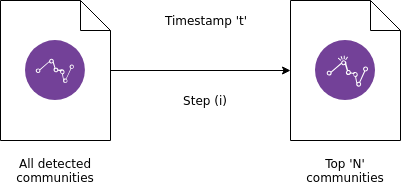
\includegraphics[width=0.5\textwidth]{framework_step_i}
	\caption{Framework: step (i)}
	\label{fig:community}
\end{figure}

In step 2(a), A sub-graph of the data-set from time-stamp $t$ is rendered according to the nodes that are present in the top $n$ communities from step one. The benefit of taking a sub-graph that has been carefully selected from the nodes that are present in top $n$ communities is that only the data that is required to track these top $n$ communities will be present in the sub-graph. A blockchain data-set can carry huge amount of transaction records and trying to use all the records every time can drastically change the behavior of the community detection algorithms as well as the framework. If all the data is selected, the framework will try to calculate communities for nodes that is not in the target communities, resulting in longer run-time and not to mention more memory consumption.

\begin{figure}[H]
	\centering
	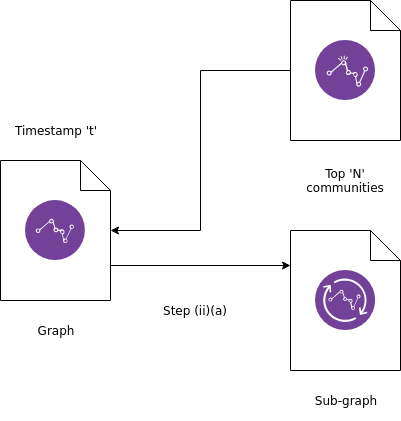
\includegraphics[width=0.5\textwidth]{framework_step_ii_a}
	\caption{Framework: step (ii)(a)}
	\label{fig:community}
\end{figure}

In the next step, two snapshots, the sub-graph from 2(a) and a snapshot of data-set from time-stamp $t+1$ are merged to create a unified snapshot of data-set for the next step. The reason for doing this is to prevent nodes from falling out from the data-set at time-stamp $t+1$. Creating a sub-graph from the data-set at time-stamp $t$ helps to reduce the number of records in the current ($t+1$ snapshot), by  adding all the nodes from time-stamp $t$ helps to keep the previous community structures intact so that with the current time-stamp, the change in the community structures are visible.

\begin{figure}[H]
	\centering
	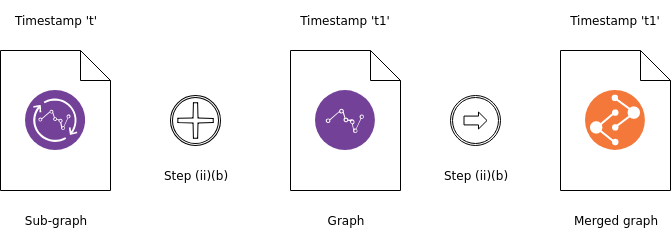
\includegraphics[width=0.7\textwidth]{framework_step_ii_b}
	\caption{Framework: step (ii)(b)}
	\label{fig:community}
\end{figure}

In step(iii), the framework repeats step one (i) on merged graph data-set to detect communities and to find out top $n$ communities from step 2(b) using the same algorithm that was used in step one for the data-set in time-stamp $t$. But, the problem is that community can change drastically over a time stamp in a network like blockchain data. As it's known that blockchain transactions are used for asset transfer, one node can just stop accepting or sending assets at the next time stamp. So to observe the change in communities, finding the similar pair of community in time-stamp $t$ and $t+1$ is important.

\begin{figure}[H]
	\centering
	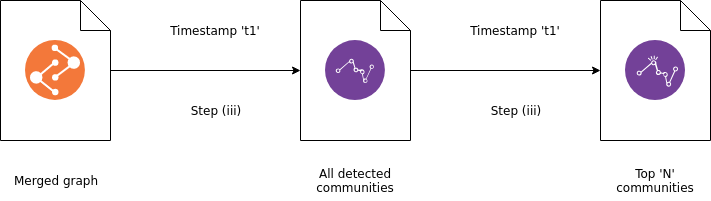
\includegraphics[width=0.7\textwidth]{framework_step_iii}
	\caption{Framework: step (iii)}
	\label{fig:community}
\end{figure}

In the last step of the framework, similarity between community pairs are drawn by the means of similarity measures described in section (\ref{vertexsimilarity}) of this thesis. Similarity measures identifies the similar communities. If top $n$ communities from time-stamp $t$ doesn't have a similar community in top $n$ communities of time-stamp $t+1$, it indicates that the community from time-stamp $t$ has lost nodes and died or became small enough to fall out from top $n$ communities. It also means that some community has been born in time-stamp $t+1$

\begin{figure}[H]
	\centering
	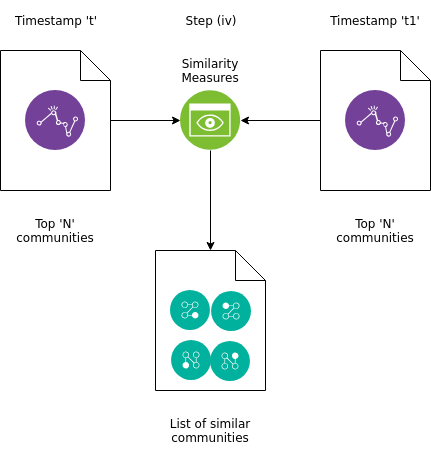
\includegraphics[width=0.5\textwidth]{framework_step_iv}
	\caption{Framework: step (iv)}
	\label{fig:community}
\end{figure}

For the scope of the thesis, implementation of the proposed framework has been done with the help of \texttt{python} programming language. Evaluation results are discussed in the next section (\ref{sec:evaluation}) in respect to run-time and memory consumption.

\section{Evaluation}\label{sec:evaluation}
Over the years different methods have been published and claimed to be the fastest and accurate. But for the scope of this thesis, three most popular and well-known algorithms are chosen to test the range of capabilities on run-time complexities and memory requirement. The obvious questions like why these particular algorithms? why not others? will be answered sequentially later in this chapter.

\subsection{Infomap}
%\textit{Infomap} uses map equation (\ref{subsec:map_equation}) from \cite{ref-43}, first introduced in 2009 by Rosvall et al. Infomap represents the community structure through two-level nomenclature based Huffman coding \cite{ref-44}. One level to distinguish communities in the network and the other, to distinguish nodes in a community. In infomap algorithm the problem of finding the best community structure is expressed as minimizing the quantity of information needed to represent some random walk in the network using this nomenclature. With a partition containing few inter-community links, the walker will probably stay longer inside the community, therefore only the second level be needed to describe its path, leading to compact representation. 
%%
Infomap algorithm starts with encoding the network into modules in a way that maximizes the amount of information about the original network. Then it sends the signal to a decoder through a channel with limited capacity. The decoder tries to decode the message and to construct a set of possible candidates for the original graph. The smaller the number of candidates, the more information about the original network has been transferred \cite{ref-49}. This algorithm runs in $\mathcal{O}(E)$, where $E$ is the number of edges. 

The main reason for choosing this algorithm for performance analysis in large-scale networks is its run-time complexity. In \cite{ref-47}, the authors stated that this algorithm works in a reasonable amount of time for detecting communities in large-scale\footnote{A network with over $1,000,000$ nodes/edges.}\label{foot:large-scale} networks. Memory consumption is also reasonable according to \cite{ref-47}. For the scope of this thesis, this algorithm's performance is being tested against blockchain transaction data to determine community structure in blockchain transactions. To determine the memory usage and run-time of this algorithm in the framework for detecting communities in blockchain data in a large network, sample data-sets from \textit{Ethereum} and \textit{Bitcoin} transactions has been used. Data have been analyzed in the same system\footnote{Intel(R) Core(TM) i5-3320M CPU @ 2.60GHz and 16 GB of RAM, with 64 bit UNIX Operating System} the framework has been implemented. 

Figure (\ref{fig:infomap_runs}) (a) shows the run-time required for infomap to detect community structures. In (a) we can observe that with the growth of the number of nodes the run-time grows but it takes less than a minute to analyze and detect communities in 2.4 Million nodes. In terms of memory, in Figure (b) for the same amount of nodes, it took only 5.1 GB of memory. In Figure, (c) and (d), run-time and memory usage reflect in respect to the number of edges. As it is seen in these figures, the run-time and memory consumption both go down on 3rd iteration because of the data-set is more connected. In general, the nodes are more connected and have more links between each other.

In terms of communities, Figure (e) and (f) show that it can detect a fair amount of communities also. As the blockchain data doesn't follow any pattern or network structure like social media so the data is more sparse than expected. Yet, there are community structures in transaction data. Infomap was able to detect communities in blockchain data-sets proving that community structures exist in blockchain data.For the scope of the thesis, the main focus is to determine run-time and memory usage for community detection algorithms in blockchain transaction data. In respect to run-time and memory usage, infomap algorithm is quite faster and has a reasonably low memory consumption. 
\vfill

% Plot run-time and memory against nodes
\begin{figure}[H]
  \centering
  \begin{minipage}[b]{0.4\textwidth}
    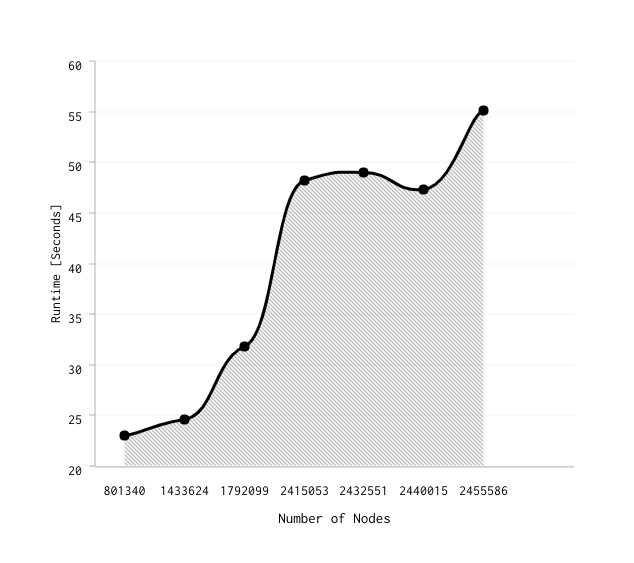
\includegraphics[width=\textwidth]{Infomap-NodesVsRuntime}
    \caption*{(a)}
  \end{minipage}
  %\hfill
  \begin{minipage}[b]{0.4\textwidth}
    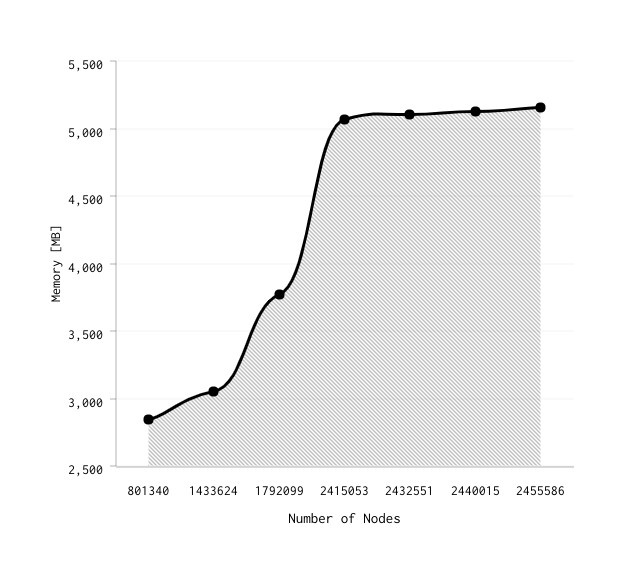
\includegraphics[width=\textwidth]{Infomap-NodesVsMemory}
    \caption*{(b)}
  \end{minipage}
  %hfill
  \begin{minipage}[b]{0.4\textwidth}
    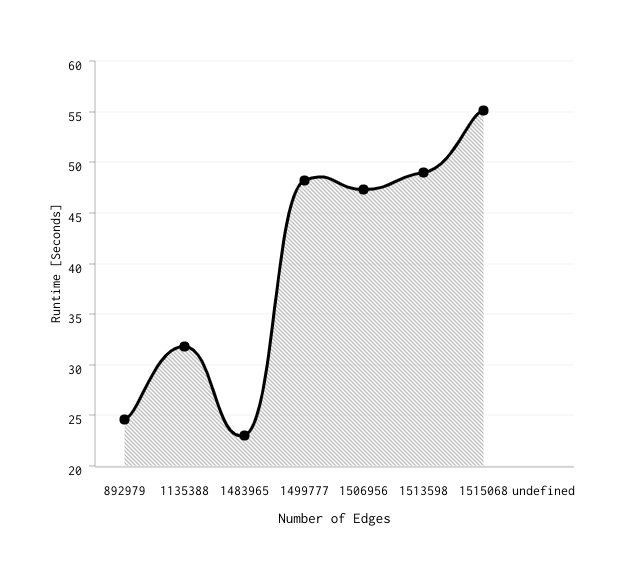
\includegraphics[width=\textwidth]{Infomap-EdgesVsRuntime}
    \caption*{(c)}
  \end{minipage}
  %\hfill
  \begin{minipage}[b]{0.4\textwidth}
    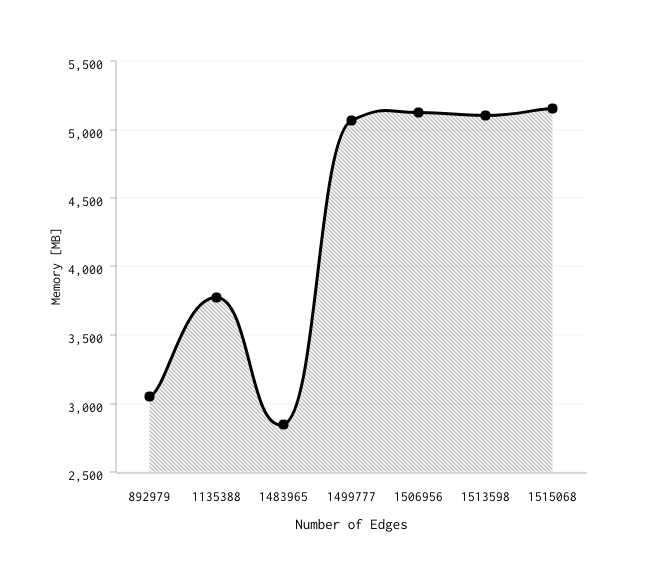
\includegraphics[width=\textwidth]{Infomap-EdgesVsMemory}
    \caption*{(d)}
  \end{minipage}
  %hfill
  \begin{minipage}[b]{0.4\textwidth}
    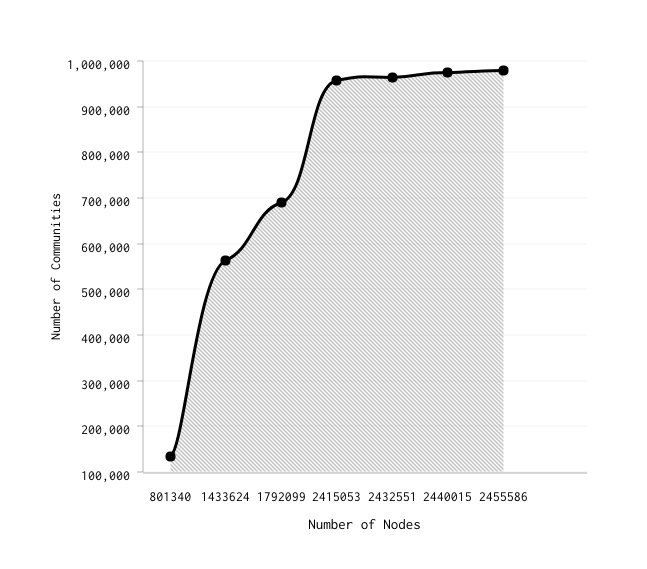
\includegraphics[width=\textwidth]{Infomap-NodesVsCommunities}
    \caption*{(e)}
  \end{minipage}
  %\hfill
  \begin{minipage}[b]{0.4\textwidth}
    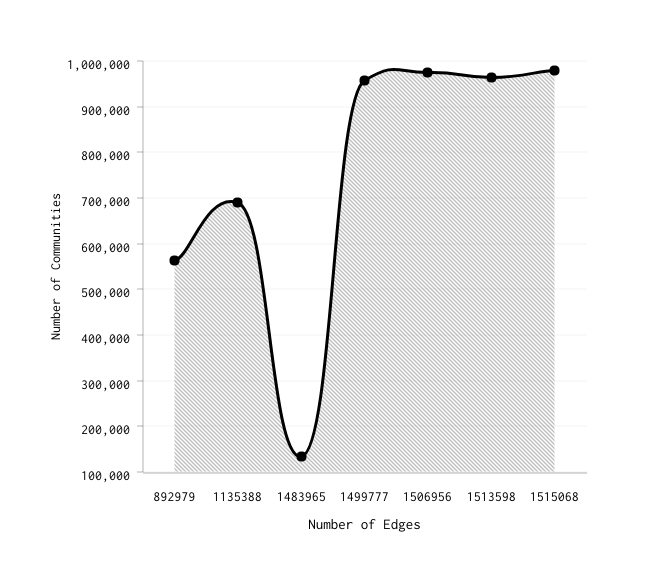
\includegraphics[width=\textwidth]{Infomap-EdgesVsCommunities}
    \caption*{(f)}
  \end{minipage}
  \caption{Infomap algorithm: (a) Run-time against number of nodes (b) Memory usage against number of nodes (c) Run-time against number of edges (d) Memory usage against number of edges (e) Number of communities against number of nodes (f) Number of communities against number of edges}
  \label{fig:infomap_runs}
\end{figure}


\subsection{Louvain}
\textit{Louvain} method (\ref{subsec:generalized_louvain}) is a heuristic method that is based on modularity optimization (\ref{subsec:modularity_maximization}). In \cite{ref-27}, Blondel et al. claimed that louvain method outperforms all other known community detection algorithm in terms of computation time. Moreover, the quality of detected communities is very good, as measured by modularity.

%Louvain algorithm is divided into two phases that are repeated iteratively. Consider a graph representing a network that has $n$ nodes. First, a different community is assigned to each node of the network. So, initially the number of communities are equal to the number of nodes. Then, for each node $i$, the neighbors $j$ of $i$ is evaluated for modularity gain if the node $i$ is removed form it's current community and placing it into the community of $j$. The node $i$ is then placed into the community with maximum gain but only if this gain is positive. If no positive gain is possible, $i$ stays in its original community.This process is applied repeatedly and sequentially for all the nodes until no further improvement can be achieved. In the second phase of the algorithm a new network is constructed whose nodes are now the communities found during the first phase. To do so, the weights of the links between the new nodes are given by the sum of the weight of the links between nodes in the corresponding two communities.
%%
Louvain method is selected for performance analysis in the large-scale network because in \cite{ref-27}, the authors stated that it outperforms any other community detection algorithm in terms of community detection. This algorithm runs in $\mathcal{O}(N \, log N)$, where $n$ is the number of nodes. For detecting community structures in large-scale blockchain networks, this algorithm can prove to be useful in terms of computation time and memory consumption.

Figure (\ref{fig:louvain-runs}) (a), shows the run-time required for detecting communities in large-scale network. Figure (a) shows the run-time with respect to number of nodes. While the number of nodes increases, the run-time increases too. In Figure (b), the memory usage has been shown in respect to same number of nodes. Louvain method has detected communities in blockchain transaction data in quite reasonable time and with a decent amount of memory usage. Louvian method can detect communities in blockchain data with 2.4 Million nodes in about 700 seconds and the memory usage is about 6.5 GB. In Figure (c) and (d), it shows the run-time and memory consumption of louvain method in respect to number of edges. In 3rd iteration, the run-time and memory usage is lower because the nodes are more closely connected in this graph.

For detected community structures, Figure (e) and (f) gives the number of detected communities in respect to number of nodes and number of edges. It is noticeable that, for over 1.4 million edges the detected communities by Louvain method is nearly 300 only and this is because of the  previously explained issue that this particular graph's nodes are more connected than the other graphs. Louvain method is quite faster and reasonable in memory consumption but with the growing number of nodes the run-time might get higher really quick.

\vfill
\pagebreak

% Plot run-time and memory against nodes
\begin{figure}[H]
  \centering
  \begin{minipage}[b]{0.4\textwidth}
    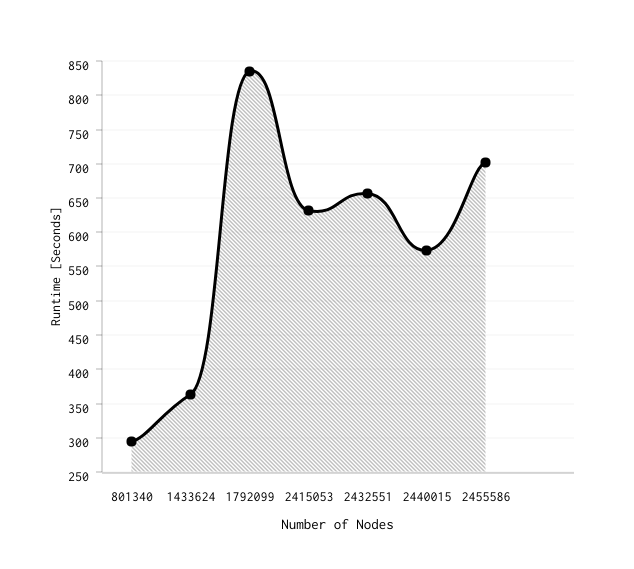
\includegraphics[width=\textwidth]{Louvain-NodesVsRuntime}
    \caption*{(a)}
  \end{minipage}
  %\hfill
  \begin{minipage}[b]{0.4\textwidth}
    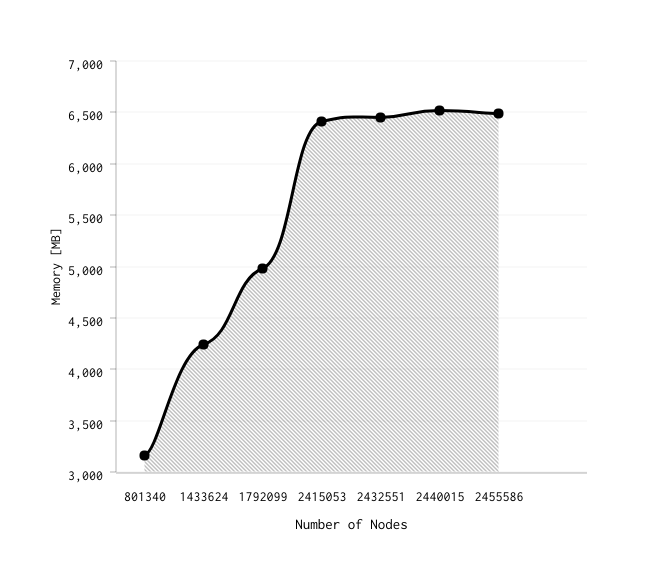
\includegraphics[width=\textwidth]{Louvain-NodesVsMemory}
    \caption*{(b)}
  \end{minipage}
%\end{figure}
%
%% Plot run-time and memory against edges
%\begin{figure}[!tbp]
%  \centering
  \begin{minipage}[b]{0.4\textwidth}
    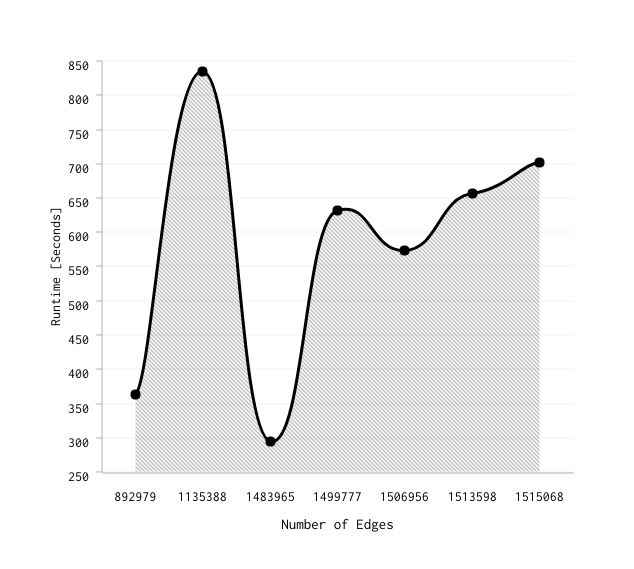
\includegraphics[width=\textwidth]{Louvain-EdgesVsRuntime}
    \caption*{(c)}
  \end{minipage}
  %\hfill
  \begin{minipage}[b]{0.4\textwidth}
    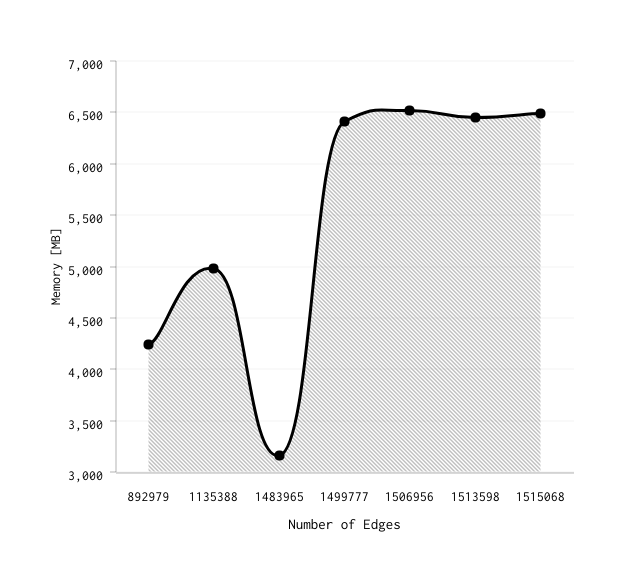
\includegraphics[width=\textwidth]{Louvain-EdgesVsMemory}
    \caption*{(d)}
  \end{minipage}
%\end{figure}
%
%% Plot detected communities
%\begin{figure}[!tbp]
%  \centering
  \begin{minipage}[b]{0.4\textwidth}
    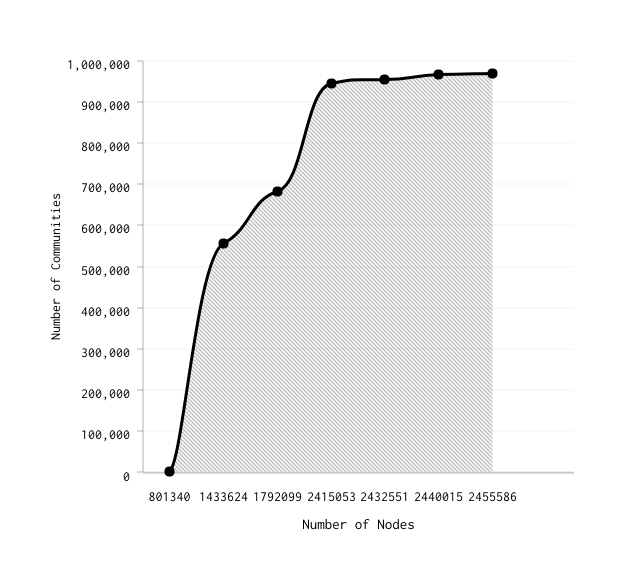
\includegraphics[width=\textwidth]{Louvain-NodesVsCommunities}
    \caption*{(e)}
  \end{minipage}
  %\hfill
  \begin{minipage}[b]{0.4\textwidth}
    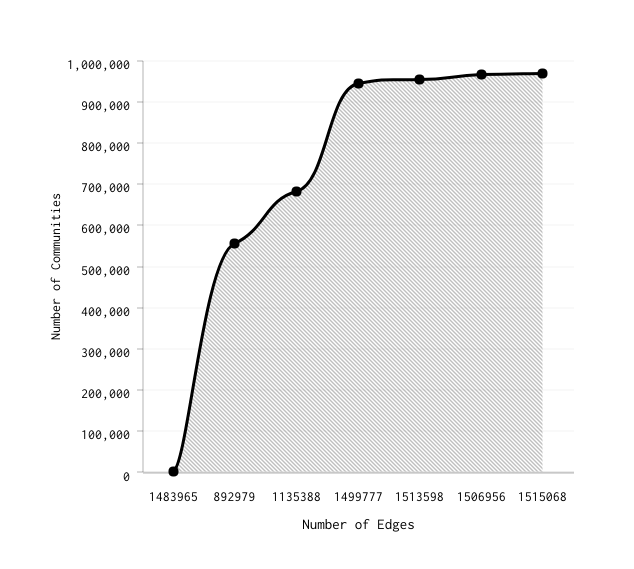
\includegraphics[width=\textwidth]{Louvain-EdgesVsCommunities}
    \caption*{(f)}
  \end{minipage}
  \caption{Louvain method algorithm: (a) run-time against number of nodes (b) memory usage against number of nodes (c) run-time against number of edges (d) Memory usage against number of edges (e) Number of communities against number of nodes (f) Number of communities against number of edges}
  \label{fig:louvain-runs}
\end{figure}

\subsection{Fast Greedy(Clauset-Newman-Moore)}
\textit{Grivan-Newman} algorithm (\ref{girvan-newman}) was proposed by M. Girvan and E. J. Newman in 2002. It is the first algorithm of the modern age of community detection in graphs \cite{ref-51}. It is a hierarchical divisive algorithm in which links are iteratively removed based on the value of their betweenness centrality (\ref{betweennesscentrality}), which expresses the number of shortest paths between a pair of nodes that pass through the link. The entire algorithm runs in worst case time $\mathcal{O}(m^2n)$.
 
%This algorithm calculates betweenness centrality using the fast algorithm of Newman \cite{ref-13}, which calculates betweenness of all $m$ edges and $n$ vertices in time $\mathcal{O}(mn)$. Because this calculation has to be repeated once for the removal of each edge, Clauset et al. in \cite{ref-31} improved girvan-newman algorithm and reduced the run-time complexity and memory consumption. The authors have used more efficient data structures to produce a set of community structures organized hierarchically, with increasing granularity \cite{ref-50}.

The fast greedy algorithm developed by Girvan-Newman, updated by Clauset et al.is promising because in \cite{ref-31} authors stated that this algorithm is capable of detecting community structures in a reasonable time with lower memory consumption. This algorithm has a complexity of $\mathcal{O}(N\,log^2N)$ \cite{ref-51}. For this reason, this algorithm is a suitable candidate for performance analysis on large-scale networks representing blockchain transactions.

In Figure (\ref{fig:CNM-runs}) (a), represents the run-time of Clauset-Newman-Moore algorithm in respect to number of nodes. In (b), it represents the memory usage of the algorithm with respect to number of nodes. In Figure (c) and (d) it represents the run-time and memory consumption in respect to number of edges. Notice that the number of maximum nodes is nearly 12000 and highest number of edges is 1.1 million. With the system described above it took nearly 500 seconds of run-time and 300 MB of memory to detect community structures in blockchain data. But beyond this nodes and edges, if the number of nodes and edges increases the run-time and memory usage increases rapidly and it takes more than 24 hours to detect community structures in a larger network graph.

In Figure (e) and (f), detected communities are shown against number of nodes and number of edges receptively. From these simulations of run-time and memory usage, it's clear that this algorithm best works with a network with small to medium networks and can detect communities in short time with low memory consumption but if the network size increases the run-time and memory consumption increases.
\vfill
\pagebreak

% Plot run-time and memory against nodes
\begin{figure}[H]
  \centering
  \begin{minipage}[b]{0.4\textwidth}
    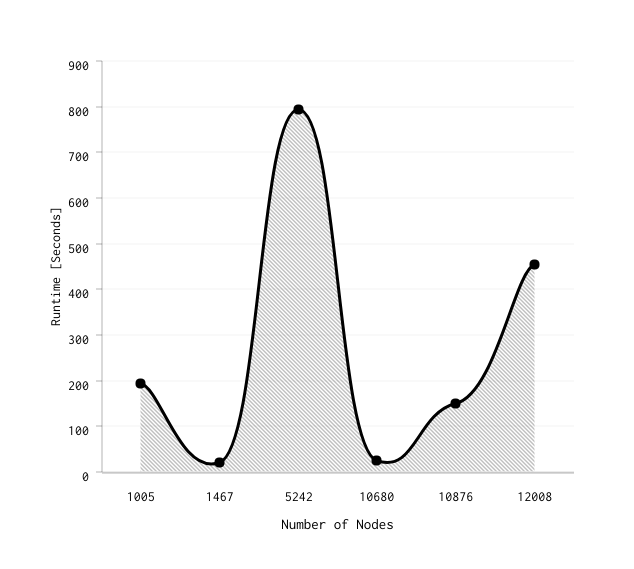
\includegraphics[width=\textwidth]{cnm-NodesVsRuntime}
    \caption*{(a)}
  \end{minipage}
  %\hfill
  \begin{minipage}[b]{0.4\textwidth}
    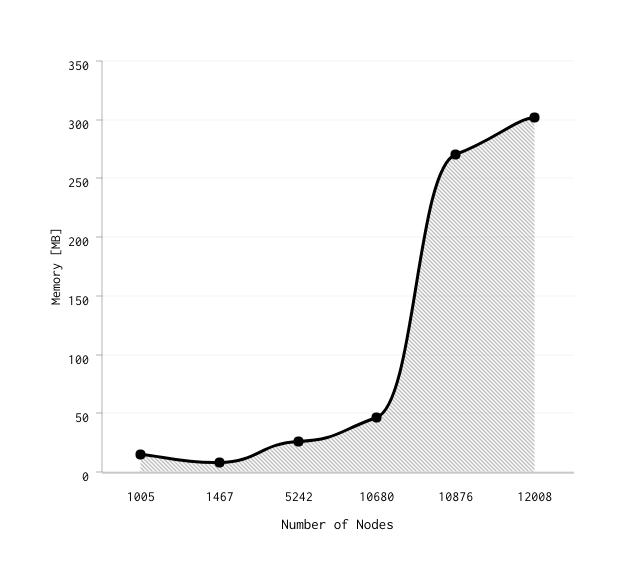
\includegraphics[width=\textwidth]{cnm-NodesVsMemory}
    \caption*{(b)}
  \end{minipage}
%\end{figure}
%
%% Plot run-time and memory against edges
%\begin{figure}[!tbp]
%  \centering
  \begin{minipage}[b]{0.4\textwidth}
    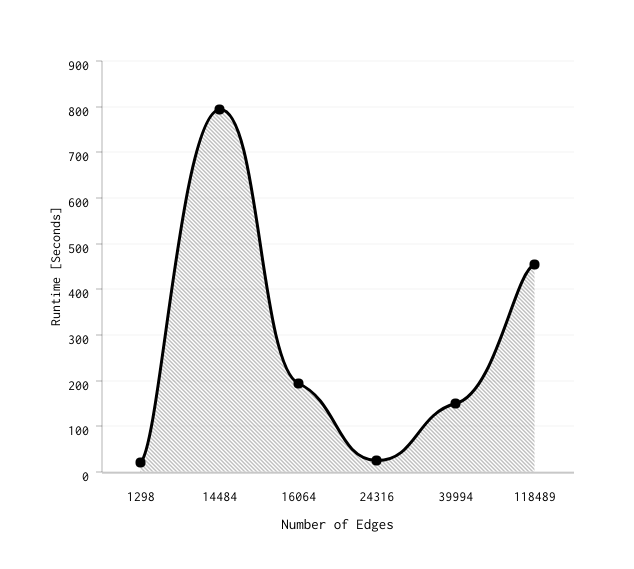
\includegraphics[width=\textwidth]{cnm-EdgesVsRuntime}
    \caption*{(c)}
  \end{minipage}
  %\hfill
  \begin{minipage}[b]{0.4\textwidth}
    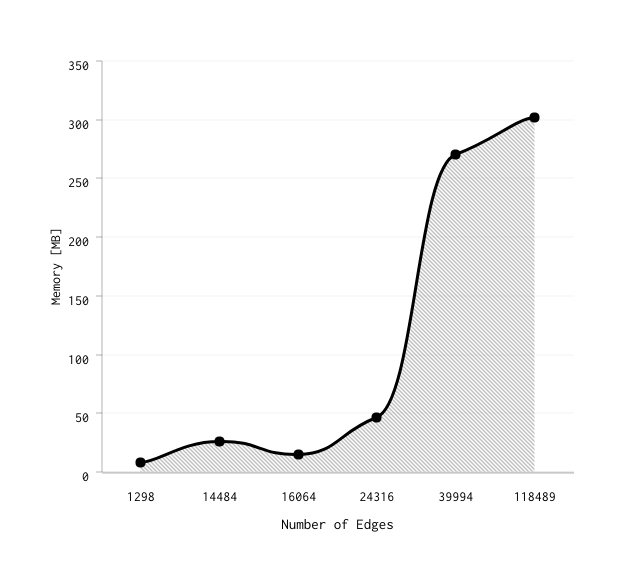
\includegraphics[width=\textwidth]{cnm-EdgesVsMemory}
    \caption*{(d)}
  \end{minipage}
%\end{figure}
%
%% Plot detected communities
%\begin{figure}[!tbp]
%  \centering
  \begin{minipage}[b]{0.4\textwidth}
    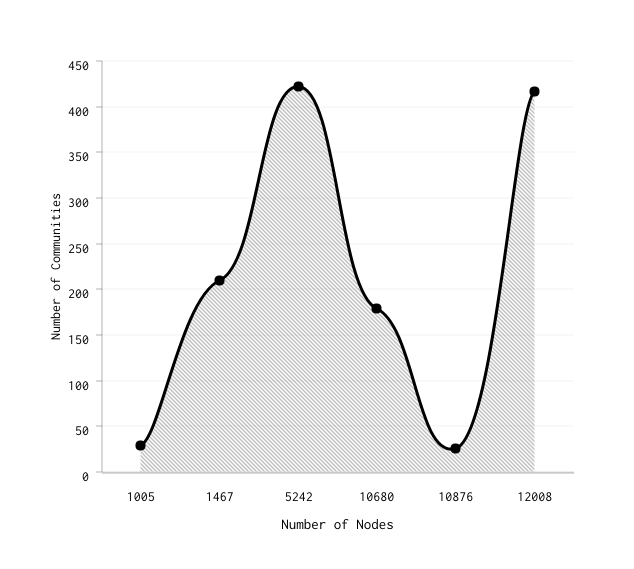
\includegraphics[width=\textwidth]{cnm-NodesVsCommunities}
    \caption*{(e)}
  \end{minipage}
  %\hfill
  \begin{minipage}[b]{0.4\textwidth}
    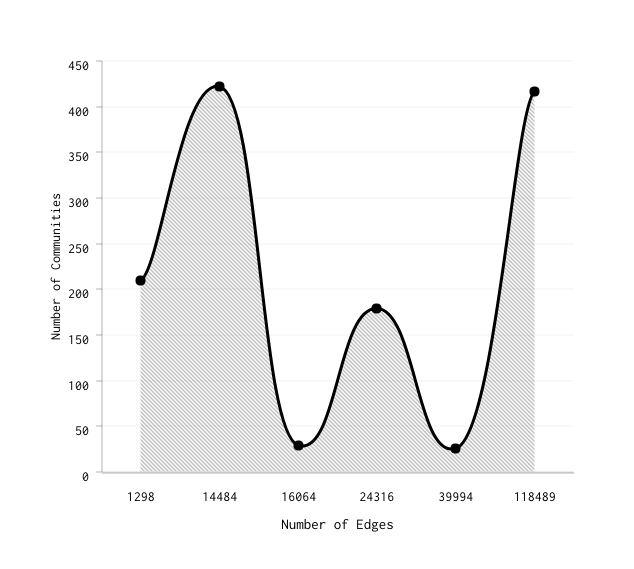
\includegraphics[width=\textwidth]{cnm-EdgesVsCommunities}
    \caption*{(f)}
  \end{minipage}
  \caption{Clauset-Newman-Moore algorithm: (a) run-time against number of nodes (b) memory usage against number of nodes (c) run-time against number of edges (d) Memory usage against number of edges (e) Number of communities against number of nodes (f) Number of communities against number of edges}
  \label{fig:CNM-runs}
\end{figure}

\vfill
\pagebreak

\section{Algorithm Comparison}
In (\ref{sec:evaluation}), the algorithms and their performance on detecting community structure are discussed with the help of blockchain data. Clauset-Newman-Moore algorithm could not deliver on the run-time and memory consumption for blockchain data as expected. On the other hand, Infomap algorithm and Louvain method algorithm seems promising for detecting community structures in blockchain transactions. So in this section, Clauset-Newman-Moore algorithm has been excluded from the comparison.

Although both the algorithms (Infomap and Louvain method) had been discussed in details, in this section a comparison of run-time and memory consumption is drawn to better understand these two algorithms' performance on blockchain data-sets.

\begin{figure}[H]
  \centering
  \begin{minipage}[b]{0.4\textwidth}
    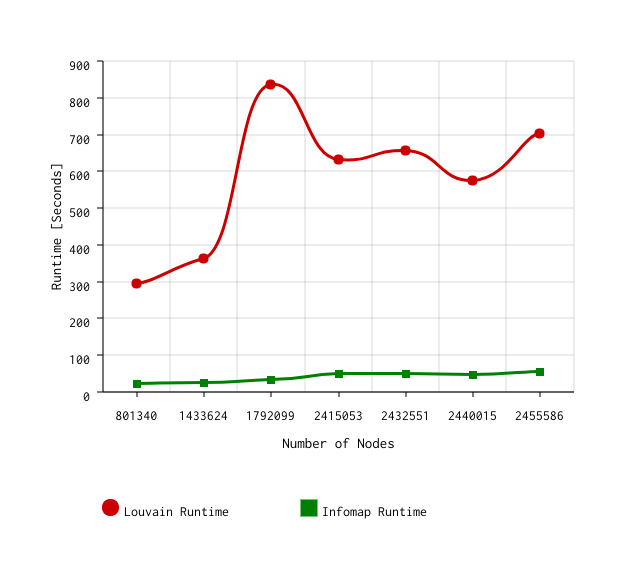
\includegraphics[width=\textwidth]{Mixed-NodesVsRuntime}
    \caption*{(a)}
  \end{minipage}
  %\hfill
  \begin{minipage}[b]{0.4\textwidth}
    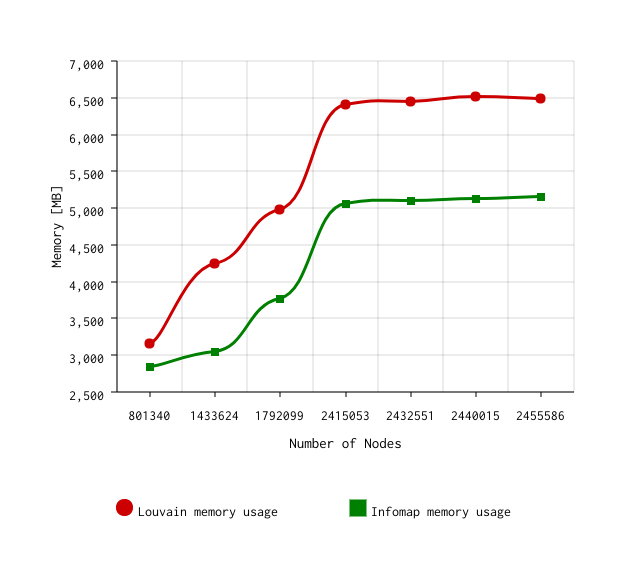
\includegraphics[width=\textwidth]{Mixed-NodesVsMemory}
    \caption*{(b)}
  \end{minipage}
  \begin{minipage}[b]{0.4\textwidth}
    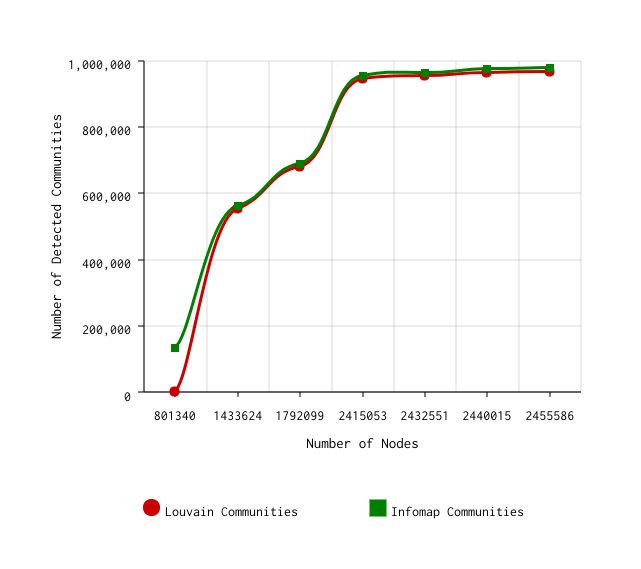
\includegraphics[width=\textwidth]{Mixed-NodesVsCommunities}
    \caption*{(c)}
  \end{minipage}
  \caption{Algorithm comparison: (a) run-time against number of nodes (b) Memory usage against number of nodes (c) Detected communities against number of nodes}
  \label{fig:algo-run-comparision}
\end{figure}

Figure (\ref{fig:algo-run-comparision}) (a), shows the run-time for both Infomap and Louvain method algorithm in respect to same amount of nodes from blockchain data-set. The same data set has been used to measure the run-time in both algorithms. In (a), Infomap algorithm runs in less than a minute for 2.4 million nodes where Louvain method runs in a little over 11 minutes. In (b), Infomap algorithm costs 5.1 GB of RAM for 2.4 million nodes where Louvain method costs 6.4 GB for the same amount of nodes from the same blockchain data-set.

Figure (\ref{fig:algo-run-comparision}) (c), shows the number of communities detected by Infomap and Louvain method algorithm from the same blockchain data-sets. Figure (c) reveals that although the first iteration of community detection gives two very different sets of results, both the algorithm detects nearly the same number of communities while the number of nodes keeps increasing. Performance of both algorithms will increase with the increase of processing power and memory of the system used to run the algorithms.

\section{Evaluation of Observation Framework}
The proposed observation framework used blockchain data with different algorithms and its performance has been evaluated so far for the detection of communities. In chapter (\ref{cha:3_concept_and_design}) section (\ref{sec:framework}) the frame work creates sub-graph of the previous graph's snapshot and merges all the nodes and edges with the current snapshot of data only if the node is present in top $n$ communities in the first graph snapshot. So after the merge, communities are detected and top $n$ communities are selected from the current (t+1) time-stamp data. A similarity measure described in chapter (\ref{cha:2_relatedwork}) is used to find the most similar community pairs to observe the changes in the community.

In Figure (\ref{fig:community_evolution_evaluation})(a) shows a single community structure from the Ethereum data of July, 2017 detected by the prototypical framework. This figure represent a single cluster of nodes that has been detect by the proposed framework. From the figure, it is observable that two nodes play very vital role in this community. Although, the community detection algorithm detected all the nodes as one community, the figure is showing different clusters because of the layout algorithm used to visualize the underlying data.

Figure (\ref{fig:community_evolution_evaluation})(b) represents the community  from (a) in the next time-stamp, in this case, the same community from next month (August, 2017). Figure (b) show the changes that happened to the previous community time interval of (t+1-t)= 1, time-stamp. It is observable that, community structure has changed in this time-stamp. The same nodes from previous time stamp was involved in more Ethereum transactions and that lead the network to create current community structure at time-stamp $t+1$.

Like figure (a) and (b), its noticeable that figure (c), (d) and (e), (f) shows the same properties of gaining more transactions and as result the community grew in size in each case. In Figure (\ref{fig:community_evolution_evaluation}), each pair of figures represents a community in two different time stamp and it's visible from the figures that all the pairs shows that the community is growing. This phenomenon is observed because of the popularity of ethereum blockchain cryptocurrency. Community could lose nodes, split into two and get merged with another community as described in section (\ref{sec:dynamic_community_algorithms}). The figures shown in this section of the thesis are only a visualization of a few communities at two different time-stamps. With the help of proposed prototypical framework it's possible to detect and observe communities as the evolve over time.

\begin{figure}[H]
  \centering
  \begin{minipage}[b]{0.4\textwidth}
    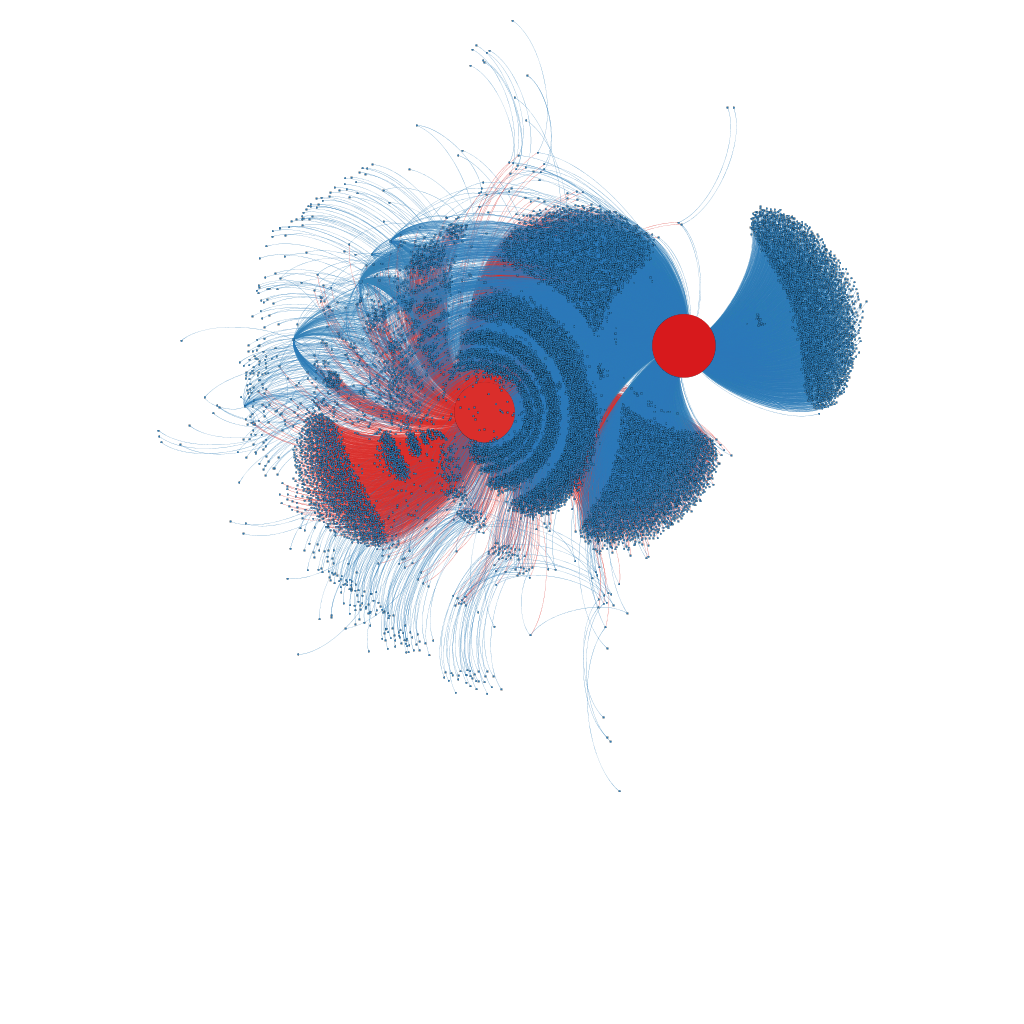
\includegraphics[width=\textwidth]{eos_community_t_1_2}
    \caption*{(a) snapshot at time $t$}
  \end{minipage}
  %\hfill
  \begin{minipage}[b]{0.4\textwidth}
    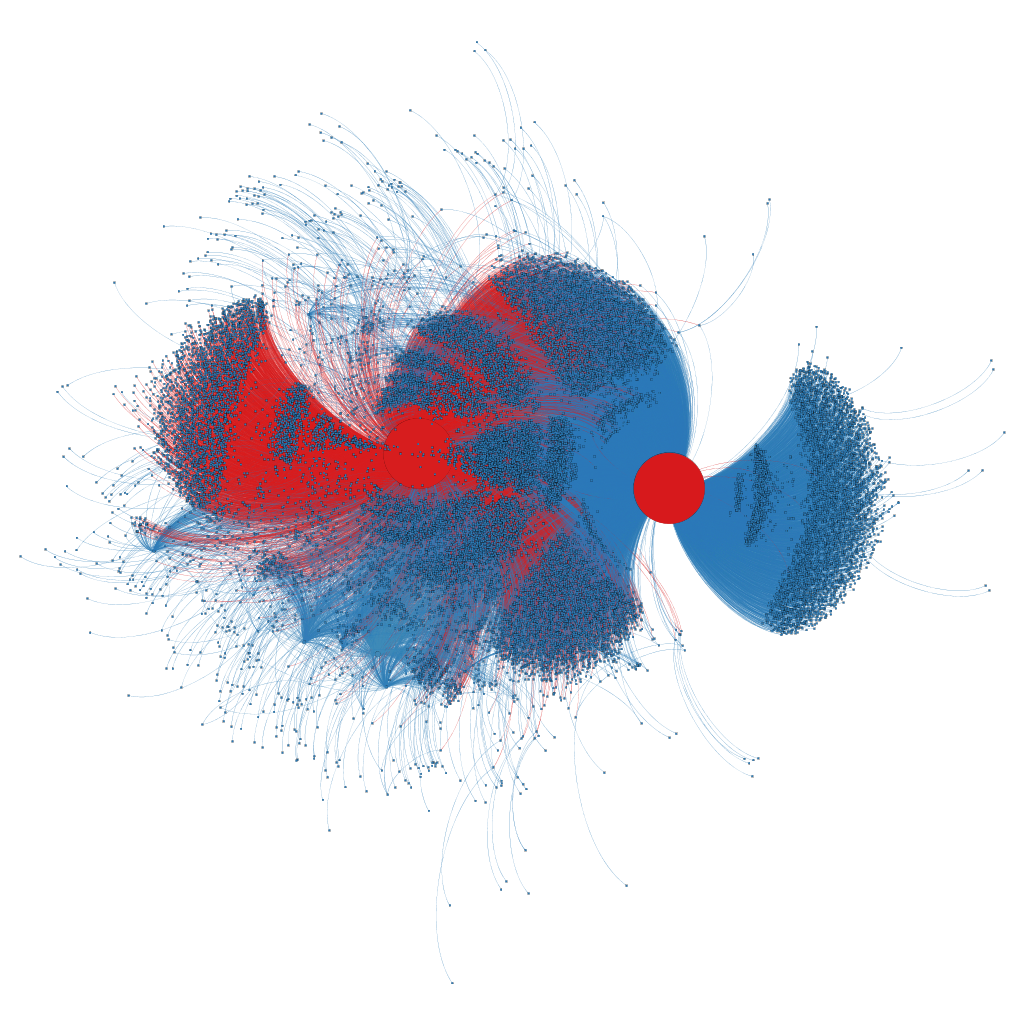
\includegraphics[width=\textwidth]{eos_community_t1_1_2}
    \caption*{(b) snapshot at time $t+1$}
  \end{minipage}
  \begin{minipage}[b]{0.4\textwidth}
    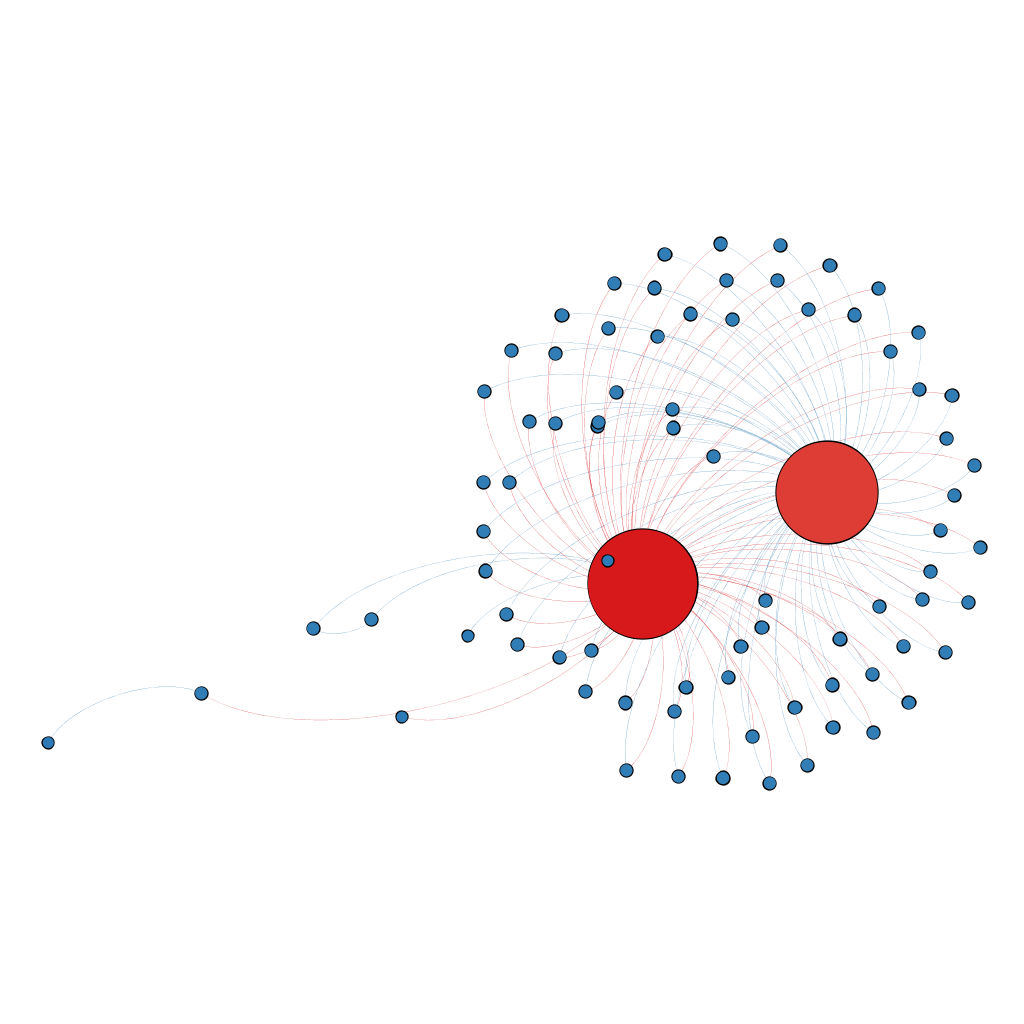
\includegraphics[width=\textwidth]{eos_community_t_15_24}
    \caption*{(c) snapshot at time $t$}
  \end{minipage}
  %\hfill
  \begin{minipage}[b]{0.4\textwidth}
    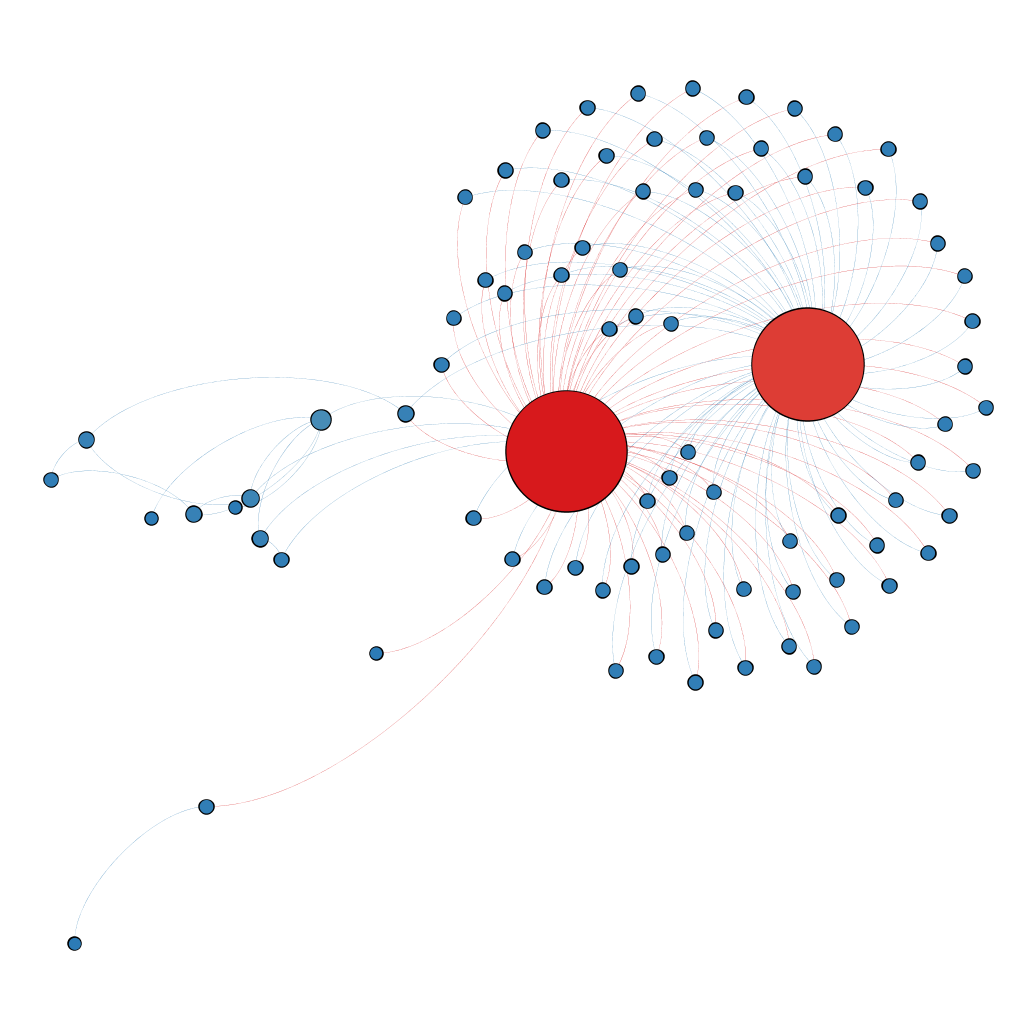
\includegraphics[width=\textwidth]{eos_community_t1_15_24}
    \caption*{(d) snapshot at time $t+1$}
  \end{minipage}
  \begin{minipage}[b]{0.4\textwidth}
    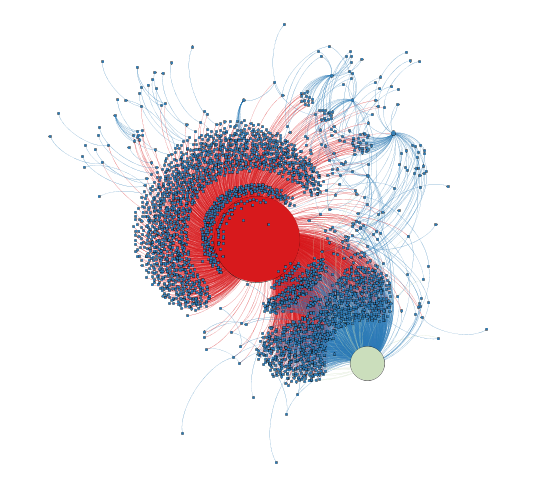
\includegraphics[width=\textwidth]{eos_community_t_6_8}
    \caption*{(e) snapshot at time $t$}
  \end{minipage}
  %\hfill
  \begin{minipage}[b]{0.4\textwidth}
    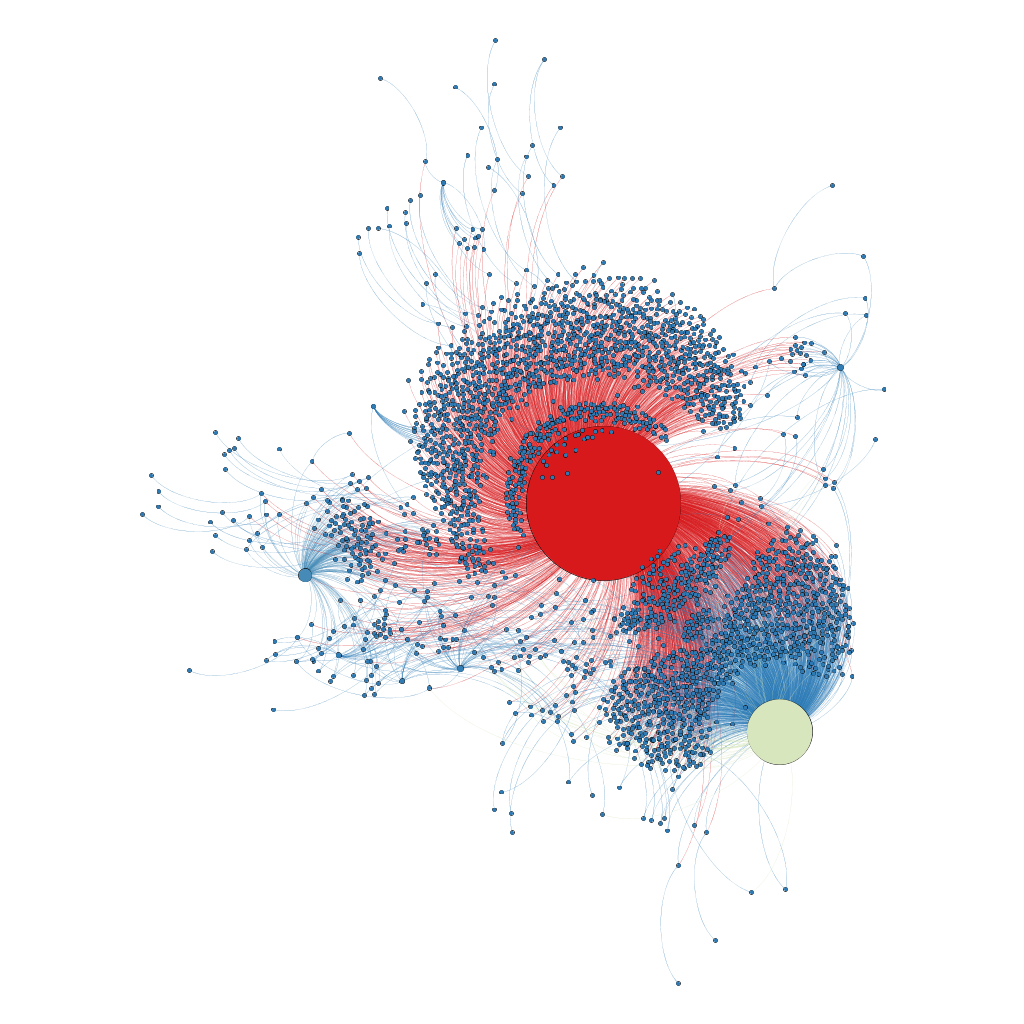
\includegraphics[width=\textwidth]{eos_community_t1_6_8}
    \caption*{(f) snapshot at time $t+1$}
  \end{minipage}
  \caption{Community evolution}
  \label{fig:community_evolution_evaluation}
\end{figure}

\chapter{Conclusion}
\label{cha:conclusion}

This thesis analyzed large-scale network (blockchain) data and built a prototypical framework for community detection and observation for blockchain transaction network. State of the art community detection techniques and their underlying algorithms have been discussed in details at the beginning of the thesis. A handful of algorithms were discussed in details from a vast number of community detection techniques for the scope of this thesis.

This thesis proposed and implemented a prototypical framework that can detect communities in blockchain transactions and observe changes afterward. This task was focused on two factors: 
\begin{itemize}
	\item run-time
	\item memory consumption
\end{itemize}
\noindent For any large-scale network data-set, it is obvious to find an optimized way to detect and track communities in blockchain data. So, the primary goal of the thesis revolved around the question - "How well an algorithm performs on large scale graph?". Secondary goal was to implement the proposed prototypical framework for observing changes in community detection. The proposed framework is implemented and evaluated in respect to run-time and memory consumption as well as detecting changes in detected communities at different time-stamps. The framework touches all the main objectives of this thesis from analyzing state of the art community detection techniques for large-scale networks, designing a prototypical framework to detect and observe changes in community to implementing and evaluating the framework.

Further study can be carried out on how to minimize the run-time even further for this framework. Determining the number of target communities will help reduce the time significantly. Proposed framework is a prototype that proves, it's possible to detect communities in blockchain data despite the anonymity of the transactions. It's possible to track communities and if necessary, a particular node's effect in the transaction network.

Blockchain gained popularity over the years and with it, the number of transaction also grew. It's a real challenge to process and analyze this huge data-set for community detection and observation. This framework is designed and implemented with the help of a medium capacity system\footnote{Intel(R) Core(TM) i5-3320M CPU @ 2.60GHz and 16 GB of RAM, with 64 bit UNIX Operating System}. Adding more feature modules to the framework is also possible and can help provide desired output depending on user's need. Framework can be further improved using a high-end system, parallel processing or distributed computing can reduce the speed and memory consumption drastically, which will help to process more nodes at any given time-stamp.



%--------------------------------------------------------------
% TABLES, FIGURES, BIBLIOGRAPHY AND APPENDICES
%--------------------------------------------------------------
\backmatter

% Lists of tables and figures
\listoftables
\listoffigures

% Bibliography
\setwidesite{}						% Set page to be wider for bibliography
\markboth{Bibliography}{Bibliography}
\label{cha:bibliography}
\printbibliography


% Use following to separate online (websites) and offline (books, papers) sources
%\printbibliography[heading=offline,filter=offline]
%\printbibliography[heading=online,filter=online]

%\begin{appendices}
%	% \chapter{Appendix 1}
\label{appendix:listing1}

\lstset{language=PHP}
\begin{lstlisting}
for($i=1; $i<123; $i++)
{
    echo "work harder! ;)";
}
\end{lstlisting}
%	% \input{content/99_appendices/a02_listings}
%	% \input{content/99_appendices/a03_listings}
%\end{appendices}

\end{document}
